
%----------------------------------------------------------------------------------
%----Präambel/Preamble-------------------------------------------------------------
%----------------------------------------------------------------------------------

\documentclass[	a4paper,
				11pt,
				DIV=11,
				bigheadings,
				idxtotoc,
				listof=totoc,	
				bibtotoc,		
				halfparskip,
				cleardoubleempty,
				oneside,
				openright]{scrartcl}
%----------------------------------------------------------------------------------

\usepackage[english]{babel}
\usepackage[T1]{fontenc}
\usepackage[utf8]{inputenc}


\usepackage{graphicx}	

\usepackage[labelfont=bf]{caption}
					
\usepackage{float}
\usepackage{wrapfig}
%\usepackage{subfigure}

\usepackage{geometry}						% Für newgeometry in Titelseite
\geometry{a4paper,left=30mm,right=20mm}

\usepackage{blindtext}
\usepackage{layout}

\PassOptionsToPackage{hyphens}{url}		
\usepackage[pdfborder={0 0 0},
			colorlinks=true, 
			linkcolor=black,
			citecolor=red,
			]{hyperref}
			
\usepackage{natbib}%numbers 				

\usepackage{pdfpages}

\usepackage{color}
\usepackage{xcolor}

\usepackage{setspace}

\usepackage{longtable}
\usepackage{multirow}
\usepackage{colortbl}

%----------------------------------------------------------------------------------
% my addition----------------------------------------------------------------------
%----------------------------------------------------------------------------------
\usepackage{chngcntr}
\counterwithin{figure}{section}

\usepackage{amsmath}

\usepackage{listings}
\usepackage{xcolor}
\definecolor{codegreen}{rgb}{0,0.6,0}
\definecolor{codegray}{rgb}{0.5,0.5,0.5}
\definecolor{codepurple}{rgb}{0.58,0,0.82}
\definecolor{backcolour}{rgb}{0.95,0.95,0.92}

\lstdefinestyle{mystyle}{
    backgroundcolor=\color{backcolour},   
    commentstyle=\color{codegreen},
    keywordstyle=\color{magenta},
    numberstyle=\tiny\color{codegray},
    stringstyle=\color{codepurple},
    basicstyle=\ttfamily\footnotesize,
    breakatwhitespace=false,         
    breaklines=true,                 
    captionpos=b,                    
    keepspaces=true,                 
    numbers=left,                    
    numbersep=5pt,                  
    showspaces=false,                
    showstringspaces=false,
    showtabs=false,                  
    tabsize=2
}

\lstset{style=mystyle}

\usepackage{pgf,tikz} % for drawing simple line charts
\usepackage{breqn}

\usepackage[edges]{forest}
\usetikzlibrary{arrows.meta}

\usetikzlibrary{shapes.geometric, arrows}
\tikzstyle{startstop} = [rectangle, rounded corners, minimum width=3cm, minimum height=1cm,text centered, draw=black, fill=red!30]
\tikzstyle{io} = [trapezium, trapezium left angle=70, trapezium right angle=110, minimum width=2cm, minimum height=1cm, text width=2.5cm, text centered, draw=black, fill=blue!30]
\tikzstyle{arrow} = [thick,->,>=stealth]
\tikzstyle{process} = [rectangle, minimum width=2.5cm, minimum height=1cm, text centered, text width=4.75cm, draw=black, fill=orange!30]
\tikzstyle{decision} = [diamond, minimum width=2.2cm, minimum height=1cm, text centered, text width=3cm, draw=black, fill=green!30]

% additional packages can be locally accessed just by downloading the library files
%\usepackage{./packages/algorithms/algorithm}
%\usepackage{./packages/algorithms/algorithmic}

\newcommand{\algorithmautorefname}{Algorithm}
\newcommand\numberthis{\addtocounter{equation}{1}\tag{\theequation}}

\usepackage{multirow}
\usepackage{subfig}
\usepackage{adjustbox}
\usepackage{epigraph}

%----------------------------------------------------------------------------------
%----Kopfzeile---------------------------------------------------------------------
%----------------------------------------------------------------------------------

\usepackage{scrpage2} 							% Aufruf KOMA-Skript für Kopfzeilen

\pagestyle{scrheadings}							% Definition der Eigenen Headerformatierung
\clearscrheadfoot 								% alle Standard-Werte und Formatierungen raus
\automark[chapter]{section}						% Kapitel und Section als Inhalt der Variablen leftmark und rightmark
\ohead{\pagemark}								% Seitenzahl auf äußerem Rand
\ihead{\ifthispageodd{\leftmark}{\rightmark}} 	% Innere Überschrift mit Kapitel bei linker Seite und Section bei rechter Seite -> geht nur in Verbindung mit
												% zweiseitigem Text wirklich sinnvoll
\setheadsepline{0.4pt} 							% Trennlinie Fußzeile und Textkörper
\setkomafont{pagehead}{\scshape}				% Schriftart in Kopfzeile, \scshape = Kapitelchen
%----Fußzeile----------------------------------------------------------------------
\setfootsepline{0.4pt} 							% Trennlinie Fußzeile und Textkörper
\setkomafont{pagefoot}{\scshape}				% Schriftart in Fußfzeile, \scshape = Kapitelchen
\ifoot{\footnotesize{John Doe}}
\ofoot{\footnotesize{Master thesis}}		
%----------------------------------------------------------------------------------

\defpagestyle{myPageStyle}{
	(0pt ,0pt)
	{\hfill\pagemark} {\hfill\pagemark} {\hfill\pagemark}
	(0pt ,0pt)	
}{
{
	(\textwidth ,0.4pt)
	\footnotesize{John Doe} \hfill \footnotesize{Master thesis}} 
	{\footnotesize{John Doe} \hfill \footnotesize{Master thesis}} 
	{\footnotesize{John Doe} \hfill \footnotesize{Master thesis}}
	(0pt ,0pt)
}


%----Farbdefinition--THI-blau------------------------------------------------------
\definecolor{haw_mag}{rgb}{0,0.112,0.47}
\addtokomafont{section}{\color{haw_mag} \rmfamily \scshape} 
\addtokomafont{subsection}{\color{haw_mag} \rmfamily}
\addtokomafont{subsubsection}{\color{haw_mag} \rmfamily}
\addtokomafont{paragraph}{\color{haw_mag} \rmfamily}
\addtokomafont{subparagraph}{\rmfamily}
%----------------------------------------------------------------------------------

\definecolor{tab_2}{RGB}{230,230,230}
\definecolor{tab_1}{RGB}{85,128,214}

%------Längenanpassung-------------------------------------------------------------
\setlength{\headsep}{10mm}						% Textabstand zur Kopfzeile
\setlength{\footskip}{15mm}						% Abstand zur Fußzeile
\setlength{\textheight}{235mm}					% Texthöhe
%----------------------------------------------------------------------------------


%----Glossar-----------------------------------------------------------------------
\usepackage[toc, acronym]{glossaries} 			
\makeglossaries	

%----------------------------------------------------------------------------------
%----Glossar-----------------------------------------------------------------------
\usepackage[intoc]{nomencl} 
\makenomenclature
%----------------------------------------------------------------------------------



\includeonly{	
	titlepage,							
	affidavit,
	acknowledgments,
	%abstractDE,
	abstractEN,
	confidentialityClause,
	glossary,
	mainpart,
	%outlook,
	%fazit,
	nomenclature,
	appendices
	}
	
			
%-------------------------------------------------------------------------------------------------------------------------------------------------------------
%----------------DOKUMENT-BEGINN---------------------------------------------------
%-------------------------------------------------------------------------------------------------------------------------------------------------------------

\begin{document}

	%\shorthandoff{"}						% Vermeidung von ungewollten Ligaturen/Avoid unwanted ligatures
	
	%----Vermeidung von Hurenkindern und Schusterjungen---------------------
	\widowpenalty=10000
	\clubpenalty=10000
	\displaywidowpenalty=10000	
	%-----------------------------------------------------------------------

	%Titelseite/title page	
	%----------Titelseite-------------------------------------------------------------

\newgeometry{height=0.9\paperheight, width=0.76\paperwidth, left=30mm, right=20mm}

\begin{titlepage}	
	%----THI+(x-company)-logo--------------------------------------------------------
\begin{figure}
      \begin{minipage}[t]{0.4\textwidth}
        \begin{flushleft}
        \colorbox{gray}{
\includegraphics[width=0.7\textwidth]{images/CES_LOGO_1C_White_normal.png}}
        \end{flushleft}
      \end{minipage}
      \hfill
      \begin{minipage}[t]{0.4\textwidth}
        \begin{flushright}
        
\includegraphics[width=0.7\textwidth]{images/thiRGB.jpg}
        \end{flushright}
      \end{minipage}
    \end{figure}
	%------------------------------------------------------------------------------
	
	\begin{center}
		\hrulefill 
	\end{center}
	
	
	\begin{center}	
		\vspace{1cm}
		
		\huge\textbf{
			Master Thesis}\\[2.5cm]
		\large
			in the study program International Automotive Engineering\\ Faculty of Electrical Engineering and Computer Science	\\ [7em]
	
		\Large\textbf{Improvement of data acquisition methods for Automotive Environmental Qualifications by combining data analytics and
compression methods}	 \\ 

	\end{center}

	\vspace{3cm}
	
	
	\begin{tabular}{lll}
		First, Last name &: & \textbf{Sajeev Saju, Pillai}	\\ [3em]
		
		Registered on &:	& 03.01.2023	\\ [1em] % issuing date
		Submitted on &:	& 31.01.2023	\\ [3em] %date of hand in
		
		First Examiner &: 	& Prof. Dr.-Ing. Armin Arnold	\\ [1em]
		Second Examiner &: 	& Prof. Dr. Ing. Andreas Hagerer	\\[3em]
		
		Company advisor &:	& Dr. Ing. Gregor Niedermayer \\ %if applicable
	\end{tabular}
	
\end{titlepage}

\restoregeometry					% include erzeugt immer eine neue Seite bei jedem Einbinden
	\cleardoublepage						% include always creates a new page
	
	\pagenumbering{Roman} 			% Römische Nummerierung der Kapitel/roman page numbering
	
	%Erklärung
	\thispagestyle{myPageStyle}
	%----------Eidesstattliche Erklärung/Affidavit--------------------------------------

\addsec{Affidavit}  % Erklärung/
I declare that I have authored this thesis independently, that I have not used other than the declared sources/resources, that I have not presented it elsewhere for examination purposes, and that I have explicitly indicated all material which has been quoted either literally or by consent from the sources used. I have marked verbatim and indirect quotations as such.	\\[2em]
	
Ingolstadt, \rule{0.3\textwidth}{0.4pt}	\\ [1.5cm]
	%\textcolor{white}{.}\qquad\qquad\qquad\qquad\quad \small (Datum) \\ [1.5cm]
	
%(Unterschrift) \\
Firstname Lastname


	\cleardoublepage
	
	%Danksagung
	\thispagestyle{myPageStyle}
	%----------Danksagung/Acknowledgments--------------------------------------------------------------
\addsec{Acknowledgments} % Danksagung/

This is the sentimental part where you get to thank all the persons who were a part of your 
thesis journey in one or the other way!
		
Sajeev Saju Pillai\\
Ingolstadt, Germany\\
January 31, 2023
	\cleardoublepage
	
	%Kurfassung/Abstract German (only for thesis written in German)
	%\thispagestyle{myPageStyle}
	%%----------Kurzfassung DEUTSCH----------------------------------------------------------------

\addsec{Kurzfassung}
Deutschsprachige Kurzfassung...
	%\cleardoublepage
	
	%Kurzfassung/Abstract Englisch (for every thesis)
	\thispagestyle{myPageStyle}
	%----------Zusammenfassung Englisch/Abstract----------------------------------------------------------------
\addsec{Abstract}

Here goes a brief description of your entire thesis.


	\cleardoublepage
	
	%Sperrvermerk/Confidentiality clause (if any)
	\thispagestyle{myPageStyle}
	%----------Sperrvermerk/Confidentiality clause------------------------------------------------------------


\addsec{Confidentiality clause} % Sperrvermerk/

Optional.\\ 
	
Ingolstadt, \rule{0.3\textwidth}{0.4pt}	\\
\textcolor{white}{.}\qquad\qquad\qquad\qquad\quad \small (Date) \\ [1.3cm]
	
(Signature) \\
Firstname Lastname

	\cleardoublepage
	
	
\nomenclature{$\sigma$}{Sigmoid function}
\nomenclature{$w$}{Neural network weights}
\nomenclature{$e$}{Euler's number}









		
	\printnomenclature
	\cleardoublepage	
	
	
%----------Glossar/Glossary-------------------------------------------------------------
% Anzeige erst auf Tools>Glossary bei jeder Änderung!!
%\newglossaryentry{abs}{name={abs},description={Absolute operation}}  



%\newacronym{d}{D}{Dimensions}
%\newacronym{rgb}{RGB}{Red Green Blue channels}
\newacronym{DUT}{DUT}{Device Under Test}




	
	\printglossaries	
	\glsaddallunused
	\cleardoublepage

	
	%Abbildungsverzeichnis/List of figures
	\thispagestyle{myPageStyle}
	\renewcommand*\listfigurename{List of figures} % Remove for German thesis
	\listoffigures
	\cleardoublepage
	
	%Tabellenverzeichnis/List of tables
	\thispagestyle{myPageStyle}
	\renewcommand*\listtablename{List of tables} % Remove for German thesis
	\listoftables
	\cleardoublepage
	
	% Inhaltsverzeichnis
	\thispagestyle{myPageStyle}
	\renewcommand{\contentsname}{Table of contents} % Remove for German thesis
	\tableofcontents
	\cleardoublepage
	\singlespacing
	
%--------------------------------------------------------------------------------	
%------Ausarbeitung--------------------------------------------------------------
%--------------------------------------------------------------------------------

	\pagenumbering{arabic} 						% Arabische Nummerierung der Kapitel/Arabic page numbering
	%----------Hauptteil/Main part of the thesis-----------------------------------------------------------
\thispagestyle{myPageStyle}
% Kapitel 1 - Einleitung
\section{Introduction}

%In diesem Kapitel wird zunächst die Motivation für dieser Arbeit dargelegt. Danach wird auch auf die Zielsetzung eingegangen, die das Thema der Arbeit fokussiert und den Grundstein für das weitere Vorgehen definiert.

\begin{quote}
    \large "The best or nothing at all." - Gottlieb Daimler
\end{quote}

This famous quote from the automotive industry resonates with every automotive enthusiast, engineer and prospective customer. From the moment we drive our cars off the dealership shop, we rely on various services in-built into the car as well as external services such maintenance checks to keep them running smoothly. Automotive industry, the world over, has come a long way since it's conception in the 19th Century and has taken giant strides in improving passenger safety, comfort and reliability. 

The automotive industry is constantly evolving and improving, which is a result of consistent improvements and developments in the automotive testing. Automotive testing is an essential aspect of the automotive industry, ensuring the safety and reliability of vehicles on the roads. With the increasing complexity of modern vehicles, it is crucial to subject them to thorough testing procedures before they are made available to consumers. This includes testing for a wide range of parameters such as performance, fuel efficiency, emissions, and crash-worthiness. Cars are becoming more and more complex products requiring a lot of effort and investments. \cite{jpower} said that: ”Automakers are investing billions of dollars into designing and building vehicles and adding technologies that consumers desire and demand”.
In order to fulfill the customer needs, modern cars, e.g., the 2014 Audi A8, have up to 80 or 90 Electronic Control Unit (ECU) for realizing the high amount of requested functions, ranging from simple interior lightning up to Advanced Driver Assistance Systems (ADAS) like Adaptive Cruise Control (ACC) \cite{Audi}.

\begin{figure}[H]
    	\centering
    	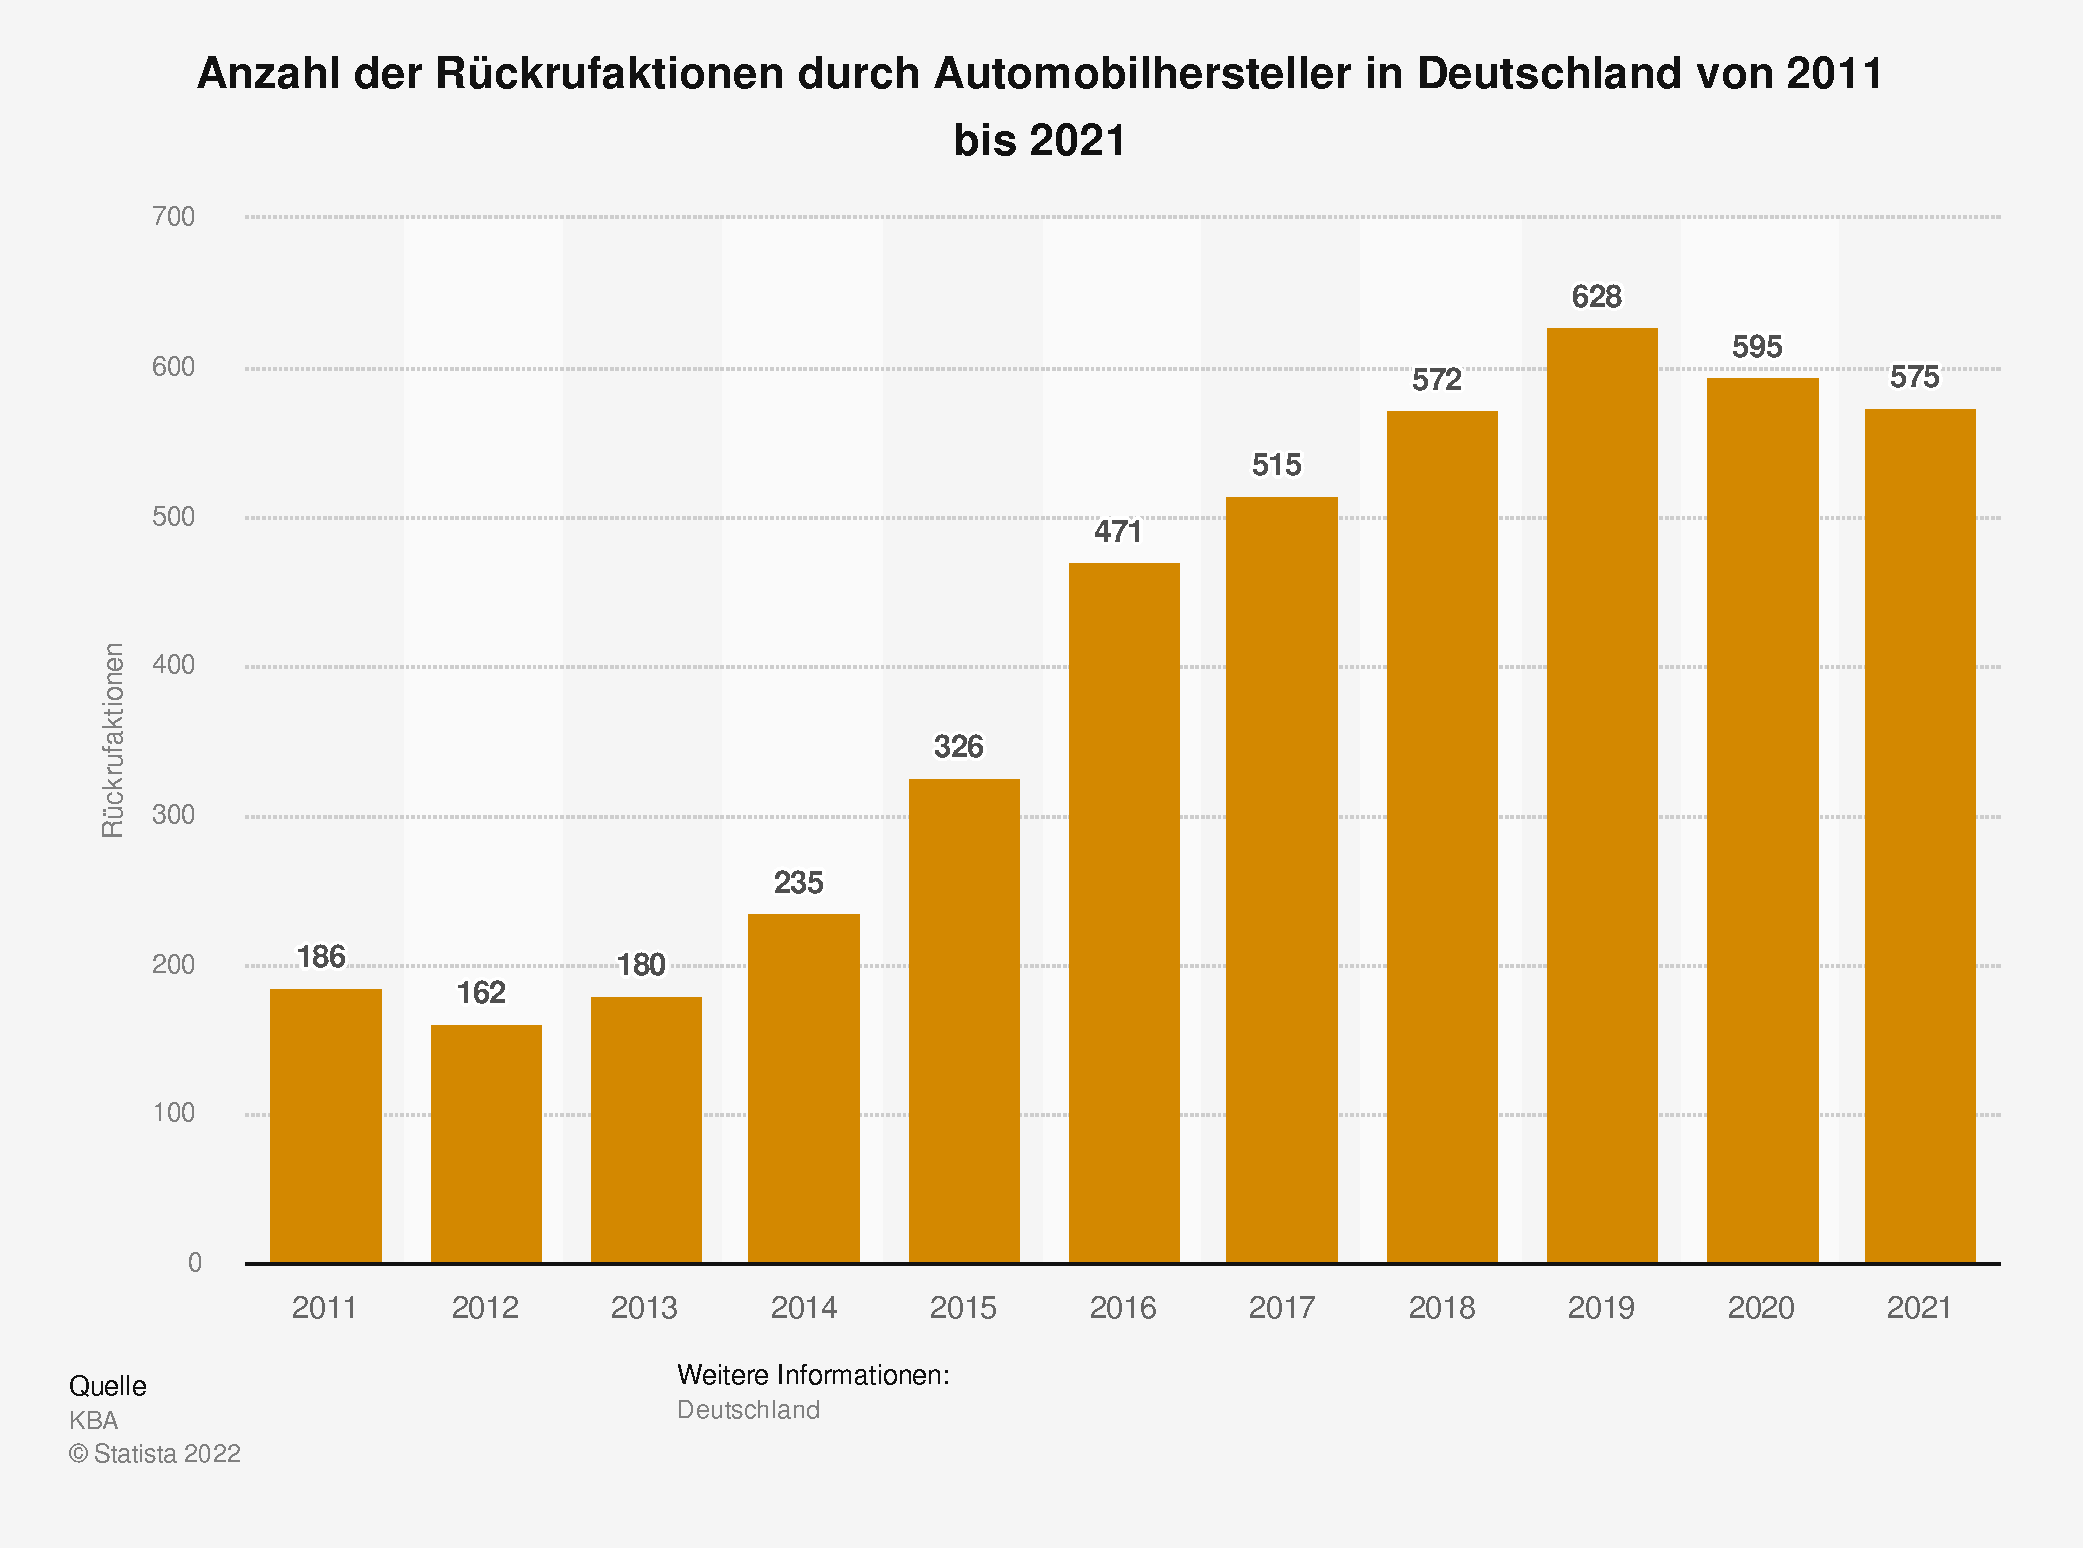
\includegraphics[width= 0.85\textwidth]{images/statistic_id1254342_rueckrufaktionen-in-der-automobilindustrie-in-deutschland-bis-2021.pdf}
    	\caption [Vehicle Recall Data]{ No. of Vehicle Recall Campaigns in Germany 2011-2021; Source: \protect\cite{KBA}}  
    	\label{fig:Statista Data}
\end{figure}
\newpage
The above diagram shows the amount of vehicle recall campaigns in Germany by Automobile Manufacturers between 2011-21. As visible, with increasing complexity and advancements in technology the amount of recalls have also increased. Testing helps manufacturers determine the necessary changes pre-production in order to incur the least damages in form of product recalls. But how do these professionals ensure that changes are necessary or unnecessary?
\textbf{By gathering data, of course!} on which this study is primarily focused on. But before diving deep into data, let's understand a bit about testing. 

Automotive testing plays a key role in the development and improvement of new technologies, such as autonomous driving and electrification. The higher the amount of comfort functions and reliability, the more complex the vehicle is. These vehicles have to undergo various tests to ensure flawless production. The value of testing is often underestimated, not understood, or mostly an afterthought, but it can be the difference between success and failure. The focus is almost always on innovations and developing the best and most sophisticated features for end users. But the questions that should be asked are  — what would these innovations and great features be like if they didn't work as expected? Not usable, not fast enough, not available, not safe — what impact would neglecting quality present? One well-known consequence is OEM mass recall — this can significantly impact people’s lives and the company reputation, plus there’s the financial damage, and the internal impact of diminished team spirit, project escalation, team dissatisfaction, productivity reduction and talent loss. In short, testing is necessary to get the desired results of innovation \cite{luxoft}.

One of the key challenges in automotive testing is simulating real-world conditions as closely as possible. This includes testing vehicles in various weather conditions, at different altitudes, and on different road surfaces. Automotive testing laboratories are equipped with advanced testing equipment and facilities to replicate these conditions and assess the performance of vehicles under a variety of scenarios. These tests fall in the scope of Environmental testing or Environmental Qualifications. Environmental testing also helps demonstrate compliance of your products with international regulations, making it easier to access global markets. Environmental testing also boosts trust in your products \cite{tüv}. In general, environmental tests demonstrate that your products have the build quality to work perfectly, no matter what the conditions. During testing, possible weaknesses can be identified and product improvements can be initiated at an early stage. 

For the purpose of environmental tests, environmental test chambers are used. They simulate various conditions that automotive components might endure in their lifetime. The systems that run such tests are called lifetime tester systems or End-of-life Test systems. Endurance tests, also known as accelerated life tests (ALTs), are a type of reliability testing used to evaluate the lifespan of a product under accelerated conditions. These tests are designed to simulate real-world usage and to identify potential failure points in a product. Endurance tests are often used in the automotive, aerospace, medical, and electronics industries to ensure the reliability of products and to identify potential failure points before they occur in the field. This can result in significant cost savings by identifying issues early in the development process, before mass production begins. In addition to identifying potential failure points, endurance testing can also be used to improve the design of a product. The results of endurance tests can be used to optimize a product's design and materials to increase its lifespan.

Overall, endurance tests or ALTs are an important aspect of product development and reliability testing, ensuring that products are safe, reliable, and able to withstand the rigors of real-world usage. They provide valuable information about a product's expected lifespan and potential failure points, helping companies to improve the design of their products and to increase customer satisfaction. This results in complex and intrinsic testing strategies which in turns results in enormous amounts of test data. Most of the data are desirable while some are undesired. One important aspect of this evolution is the development of effective methods for acquiring data about the environmental performance of vehicles. Environmental endurance tests for automotive components are critical for ensuring the safety and reliability of vehicles on the road. These tests simulate real-world conditions such as extreme temperatures, humidity, and vibration to evaluate the lifespan of components and identify potential failure points. However, the data generated from these tests can be large and complex, making it challenging to manage and analyze. One common problem faced when working with large data sets from environmental endurance tests is the difficulty in identifying patterns or trends in the data. Another problem is that the data can be highly variable, making it difficult to establish clear cause-and-effect relationships. Additionally, the data obtained from these tests is often not in a format that is easy to work with, requiring data processing and cleaning to be able to analyze them. This can be a time-consuming and tedious process.

The size of data log files generated from environmental endurance tests can be quite large, and managing and analyzing them can be a challenge. Here are a few ways to tackle the problem of large data log files:

\begin{itemize}
    \item Data Compression
    \item Data Sub-sampling
    \item Data Filtering
    \item Data management tools
    \item Data archiving
\end{itemize}

This thesis would study some of the above mentioned methods apart from combining approaches of data analytics and data reduction to enhance the efficiency and accuracy of data acquisition for automotive environmental qualifications.

\subsection{Motivation}
%https://www.cbtnews.com/consumer-reports-releases-annual-reliability-rankings-for-auto-brands/
According to \cite{viewpoint} "Reliability testing, aka endurance or durability testing, runs the part through many hours of use while monitoring (sometimes continuously, sometimes periodically), the performance of the part. Different than design validation, the part is usually not subject to a wide range of extreme conditions to look for corner cases, but rather subjected to “normal” operation in an accelerated fashion. Note that “normal” might not imply static operating conditions. Rather the part might be cycled through a range of conditions seen in normal usage, such as back and forth motion for a car seat cushion, or -120 C to +120 C temperature cycling for a satellite part orbiting the earth. Parts are often run to failure or to degraded performance to verify that one design is better or worse than another. Sometimes, the performance measurements are coupled with an analysis of the failure mode(s). Other times, this failure mode and effects analysis (FMEA) is done without reviewing any measurements taken during the cycling, implying that the reliability test system controls the automated cycling without assessing operation. However, starting in the early ~2000s, data collection during cycling has become nearly universal."

When the part is expensive or the cost of failure of the part is expensive the hardware or DUT is more likely to go through non-negligible reliability testing. Often such tests require to mimic the lifetime behaviour of the equipment in discussion. The result is potentially massive amount of data. One could imagine such tests to often run for 100s of hours on average. Depending on the data being collected, and it's type the accumulated data could often end up being 100s of GBs of data. Scaling up the tests and the no. of DUTs tested, a couple of these tests are sufficient to overload the storage infrastructures of companies performing such tests. As explained in previous section, there is great need for efficiently managing the data in order to efficiently reduce the costs but more importantly deliver precise and tangible data to the client.

The Business Center Verification and Validation at CES is responsible for such endurance / life cycle tests. The HiL test-benches are capable of testing up to 8 DUTs at a time. The average duration for such tests are ~250 hours and above. This leads to an accumulation of data to the tune of approx. 500 gb per project. Considering the increasing demands of testing in modern automotive, the massive size of data is a pain point for the IT infrastructure. Apart from the sheer size of data costing the company in terms of storage space and it's scaling, managing such a huge set of data would be a nightmare if the client requests only specific section of data as final result from the tests. This scenario immediately brings two requirements to one's attention :

\begin{itemize}
    \item Reduction of data size
    \item Making sense of the acquired data
\end{itemize} 

The above requirements are the motivation behind the scientific study undertaken with this thesis where the focus lies on designing an algorithm that reduces the size of the acquired data while also attempting to improve the efficiency of data acquisition. 


\begin{comment}
    \begin{figure}[H]
    	\centering
    	\includegraphics[width= 0.95\textwidth]{}
    	\caption[Verlauf der Anzahl an Todesopfer im deutschen Straßenverkehr von 1953 bis 2016 in Kombination mit Einführung von Fahrerassistenzsystemen]{Statistik der Todesfälle im deutschen Straßenverkehr mit Einführungsdaten von FAS; Quelle: Statistisches Bundesamt \protect\cite{sba}}  
    	\label{fig:Statista Data}
    \end{figure}
\end{comment}
\begin{comment}



















\subsection{Zielsetzung}
\glqq Die Automatisierung der Fahrzeugführung verändert die Anforderungen an das kognitive System des Autofahrers grundlegend. Um daraus keine Gefahren entstehen zu lassen, sind noch zahlreiche Fragen offen.\grqq{} \cite{schlott}. Schlott trifft diese Aussage um die kritischen Aspekte der hochautomatisierten Fahrt zu beleuchten und um auf mögliche Risiken hinzuweisen. 

Diese Arbeit befasst sich sowohl mit der Erhebung der technischen Grundlagen, als auch mit dem menschlichen Informationsverarbeitungsprozess. Die Erkenntnisse aus den einzelnen Bereichen werden aggregiert und miteinander verknüpft, um somit die Basis für ein umfassendes HMI-Konzept zu generieren. Dieses soll die benötigten Informationen aller Automatisierungsstufen zur Förderung des Vertrauens in das Gesamtsystem und Aufrechterhaltung des Situationsbewussteins darstellt, um den Fahrer zu unterstützen. 

Das auszuarbeitende Konzept soll in einem Entwicklungsfahrzeug, weitere Details siehe \autoref{sec:entfahr}, eingesetzt werden und umfasst somit nur die Automatisierungsstufen 0 bis 3, da zum aktuellen Zeitpunkt noch keine aktiven Fahrerassistenzsysteme für höhere Automatisierungsstufen zur Verfügung stehen. Dazu wird folgende Forschungsfrage gestellt: \\

\begin{tabular}{p{0.3cm} p{0.5cm} p{13cm} p{0.5cm}}
	& \textbf{RQ}	& Können die bla bla? & \\
\end{tabular}
\vspace{1em} 

Es wird angenommen, dass sich das Informationsbedürfnis des Fahrers über die Automatisierungsstufen unterschiedlich verhält und eine sich dynamisch veränderbare Anzeige gefordert wird. Daraus lassen sich folgende Hypothesen ableiten: \\

\begin{longtable}{p{0.3cm} p{0.5cm} p{13cm} p{0.5cm}}
	& \textbf{H1}	& Je höher, desto geringer. & \\
	& & & \\
	& \textbf{H2}	& Bla bla, bla bla. & \\
	& & & \\
	& \textbf{H3}	& Bla bla, bla bla. & \\
\end{longtable}
\end{comment}			% 1. Einleitung/Introduction and problem statement
\newpage

\thispagestyle{myPageStyle}
% Kapitel 2 - Related Work / Literaturanalyse
\section{System Introduction}\label{sec:RelatedWork}

The previous chapter aimed at shedding light on the process of testing in the modern automotive industry and the problems faced as a result. It is important to understand the systems being dealt with before setting any fixed goals. It is a crucial pre-requisite for setting goals as the adaptation and corresponding fine tuning would be a direct by-product of this. This section introduces the existing approach and methods to tackle the aforementioned problem of enormous data size. 
%-------------------------------------------------------------------------------------------------------------------------------------------------------------

\subsection{Introduction to Hardware} \label{sec:hardware}
 As mentioned earlier on, this thesis deals with Life Time Tester systems for Environmental Qualifications. The life cycles of the test specimens are simulated and the are simulated and thus the behaviour over the service life is determined. Various properties such as current or voltage can be monitored. Furthermore, it is possible, for example, to combine the test facility with a climate chamber for testing temperature cycles. 

Testing is carried out within the framework of a Qualification Program (\textbf{QP}) according to certain specifications. Generally speaking, there are two basic work packages that fall under the heading of testing. The first is the so-called Design Verification (\textbf{DV}). This generally includes all theoretical processes that are intended to ensure that all design requirements for the product are fulfilled. The DV is followed by the so-called product validation (PV). Here, the functionality of the product including the requirements is tested in practical test procedures. In the context of a \textbf{QP}(Qualification Program), one also speaks of a so-called DV/PV. Many hardware components for controlling the inputs for the data acquisition devices are interconnected, the most important of which are explained here. 

The basic framework for the test system is a 19-inch test rack in which all components are integrated. A photo of the front view of the test system can be seen in \hyperref[fig:Testrack]{Figure 2}. The test rack has a height of approx. 1.50 m, on which the test PC stands, and it is divided into individual height units (HE) according to the rack standard. The test units can be tested with the standard bus systems CAN (FD), LIN, Ethernet and Flexray. A total of eight \gls{DUT}s can be connected to the test rack at the same time. can be connected to the test rack at the same time. They are connected to the test system via 108-pole Harting industrial connectors. These are fully assigned and, depending on the project configuration, a different number of data lines and bus systems are required. In total, the following data bus communications are possible :

\begin{itemize}
    \item 7 x CAN
    \item 4 x LIN
    \item 9 x Ethernet
    \item 4 x Flexray
\end{itemize}

\begin{figure}
  \centering
  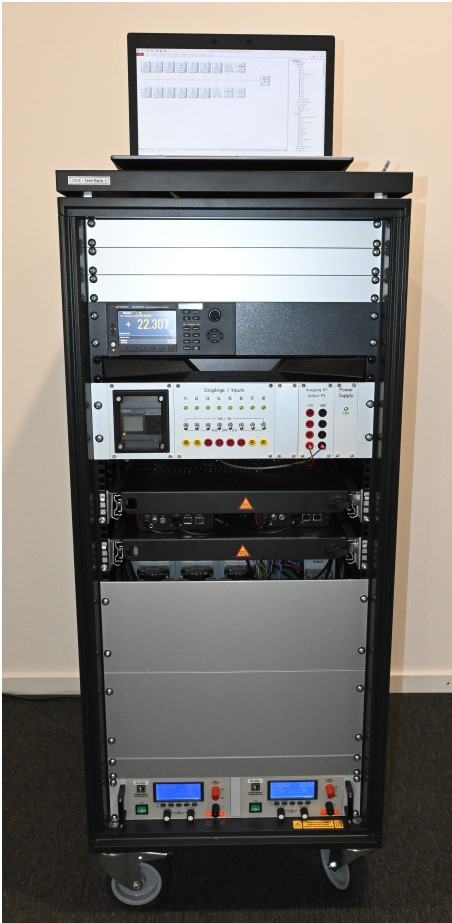
\includegraphics[width= 0.6\textwidth]{images/Testrack.jpg}
  \caption{19 inch "wide" Testrack}
  \label{fig:Testrack}
\end{figure}

In addition, individual measuring channels for the voltage and current measurements of the DUTs are integrated, for example. The supply voltages for Kl. 15 (switched positive from ignition lock) and Kl.30 (positive line from battery) according to DIN 72552 can be modelled including the necessary ground (GND) lines. 

One signal LED per DUT is integrated for each connected terminal. There is a power supply unit at the bottom of the Testrack which feeds in the DC voltage for all the DUTs. \begin{comment}
The power supply units are PSI 5000A DC Laboratory Power Supply from Elektro-Automatik [12], which is shown at the bottom of Figure 2.2. Figure 2.2 at the bottom.
\end{comment}
In addition, the front panel contains the connection for a PT-1000 temperature sensor, which is responsible for measuring an external chamber temperature, and a connection for an external trigger. The central measuring unit of the test system is the Keysight Data Acquisition System. This is integrated into the front of the test rack. It can be seen in \hyperref[fig:Testrack]{Figure 2} in the upper part with the current temperature display. Three different measuring cards, which are connected to the test rack via 50-pin Sub-D plugs to the test rack, enable measurements of different amplitudes/sizes.

The current is measured for each DUT via a shunt resistor R\textsubscript{s}. The voltage drop U\textsubscript{s} at the shunt is measured via a measuring line and the corresponding current is calculated according to Ohm's law (see equation 2.1), the corresponding current is calculated.

\begin{equation}
I_s= \frac{U_s}{R_s}\
\end{equation}

The individual DUTs are switched via automotive relays. If the relay is closed, a voltage drop can be measured at the shunt resistor and the corresponding current at the DUT can be calculated via equation 2.1. Two low-power LEDs (for terminal 15 and terminal 30) indicate to the operator whether a DUT is connected. The hardware equipment for controlling the data buses in the form of frame, load and error generation comes from Vector Informatik GmbH. The following network interfaces are included in each test system in a 19 inch rack system:
\begin{itemize}
    \item 4 x VN640 ( CAN, LIN, FlexRay)
    \item 2 x VN5620 (Ethernet, CAN)
    \item 1 x VN1630 A (CAN, LIN)
\end{itemize}

All Vector hardware is usually integrated horizontally in the lower drawer system shown in \hyperref[fig:Testrack]{Figure 2}. The individual data sheets of the Vector hardware are available on the manufacturer's homepage. The connection to the test computer is made via a serial USB interface. For this purpose, another pull-out height unit is equipped with USB hubs for communication of the Vector control units with the test computer. For each Vector control unit, the individual channels can be individually configured in the so-called \emph{Vector-Hardware-Configuration}.

A portable test computer is available for each of the four test systems. The development and test software CANoe from Vector Informatik and further test automation software are essential for carrying out the tests. 

%Riener \cite{riener} hat sich die Frage gestellt, was sich aus dem Einsatz von Autopilotensystemen in der Luftfahrt für den Bereich des (teil)automatisierten Fahrens in der Automobilindustrie übertragen/lernen lässt und was man für die Gestaltung der Interaktion übertragbar machen könnte. usw. usw.
%Gold et al. thematisierten die Frage, ``zu welchem Zeitpunkt, vor dem Auftreten einer Systemgrenze, muss das FAS die Aufmerksamkeit des Fahrers auf sich ziehen, um eine erfolgreiche Übernahme durch den Fahrer auch dann sicherzustellen, wenn er sich nicht im Loop befindet.'' \cite{gold} %
Hierzu wurde eine Studie mit 32 Probanden in einem High-Fidelity-Fahrsimulator bei BMW durchgeführt. Das Szenario beschreibt eine Fahrt mit 120 km/h auf einer dreispurigen Autobahn, bei der das vorausfahrende Auto einen Unfall verursacht und somit den Fahrer zu handeln zwingt. 17 Probanden haben dieses Szenario als Referenz manuell durchfahren, wobei der Unfall zum Einen fünf Sekunden, zum Anderen 7 Sekunden entfernt war. Die gleichen Zeiten wurden für die Probanden der hochautomatisierten Zeit eingehalten um die Übergabe einzuleiten.  

Folgende Ergebnisse konnten aus dieser Studie gezogen werden:
\begin{itemize}
	\item[1.] Die geringe Zeit bis zur Übernahme lässt die Probanden schneller zu einer Entscheidung und Reaktion kommen, dennoch ist deren Qualität schlecht.
	\item[2.] Mit der sich verringernden Zeit bis zur Übernahme nehmen die Kontrollblicke in Spiegel und über die Schulter ab, hingegen nimmt die Beschleunigung zu, sowie auch das Betätigen der Bremse.
	\item[3.] Vergleicht man die Probanden aus der Referenzfahrt und der hochautomatisierten Fahrt, wird deutlich, dass bei den Probanden der hochautomatisierten Fahrt bis zu dreimal so hohe Beschleunigungen erzielt wurden. Auch werden hier viele plötzliche Bremsmanöver durchgeführt. 
\end{itemize}

Die Studie belegt unter diesen experimentellen Bedingungen, dass bei vollständiger Ablenkung des Fahrers bei hochautomatisierter Fahrt noch bei sieben Sekunden Übernahmezeit ein Automatisierungseffekt auftritt. Das bedeutet, dass der Fahrer durch die fahr-fremde Nebentätigkeit stark abgelenkt ist und der automatisierten Fahrt vertraut. Dies führt zu solchen Reaktionen bei unerwarteter Bekanntmachung von Übernahmen. 







\newpage

\subsection{Introduction to Software}

The basis for the environmental qualification tests is laid in Vector CANoe by means of a configuration (.cfg-file). It allows to analyse a multi-bus communication of ECUs or entire systems.
CANoe performs following functions \cite{pd} : 
\begin{itemize}
    \item Creation of simulation models which simulate the behavior of the ECUs
    \item Graphic and text based analysis windows are provided for evaluating the results
    \item Create custom interfaces to control the simulation and tests or to display the analysis data
    \item Ease of programming through the CAN Access Programming Language (CAPL) to support simulation, analysis and testing
\end{itemize}

In the measurement setup, the data flow for the individual bus communications is graphically displayed and configured. The typical measurement setup of a CANoe configuration can be found below. In the measurement setup, so-called CAPL program nodes can be inserted, which are represented by the individual grey boxes. 


\begin{figure}[H]
	\centering
	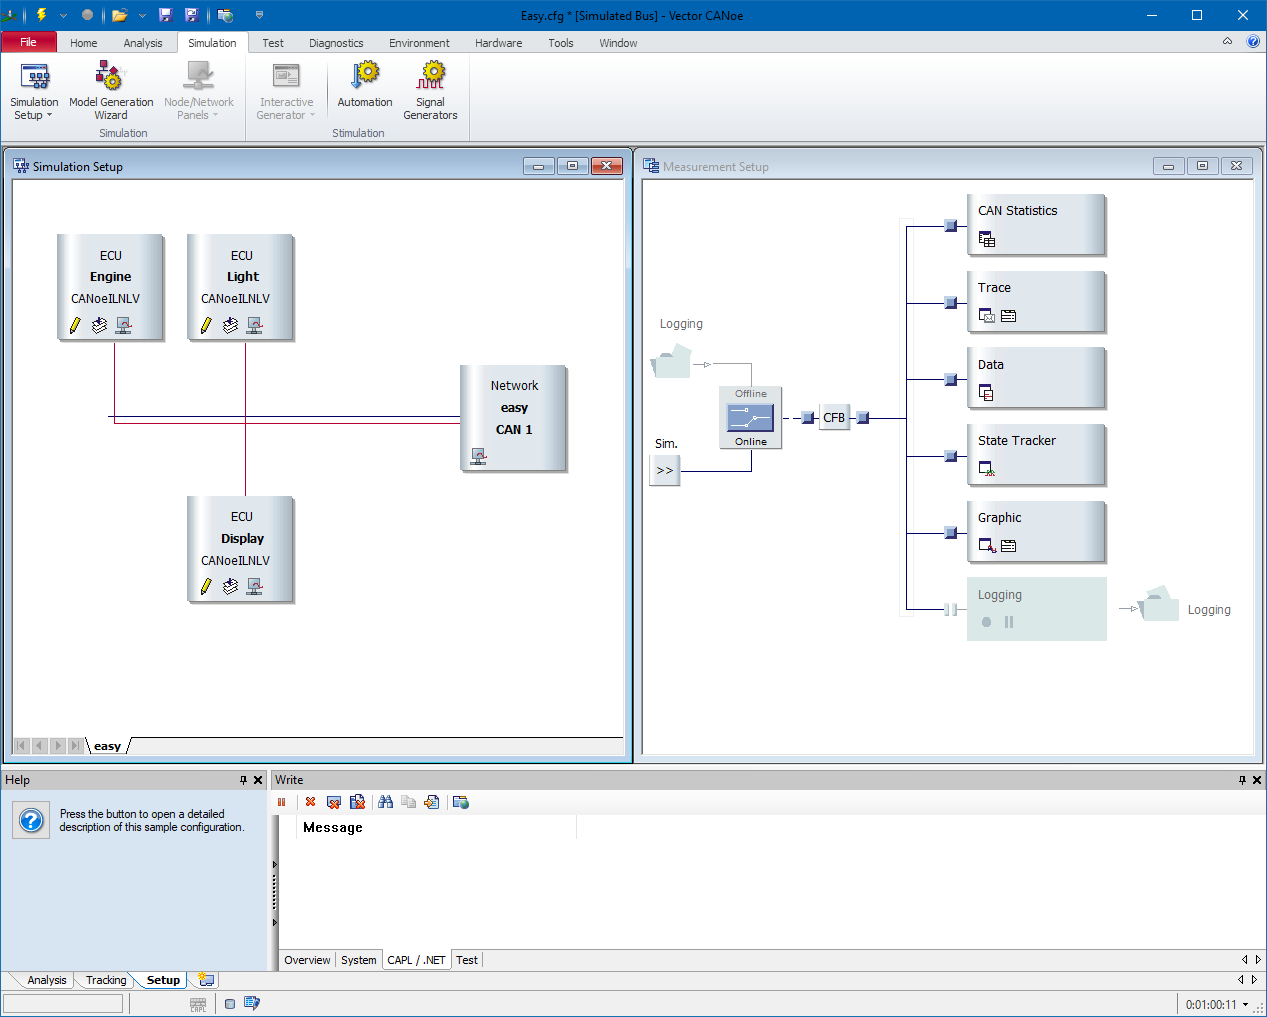
\includegraphics[width= 0.9\textwidth]{images/CANoe_Simulation_setup.png}
	\caption[CANoe Simulation and Measurement Setup]{CANoe Measurement Setup \cite{CANOE} } 
	\label{fig:Measurement Setup}
\end{figure}

Furthermore, analysis windows can be inserted with which the data can be displayed in different ways (e.g. as a graphic display of signal curves or as a display of signal values). In the so-called trace window, bus activities such as the sending of messages or error frames are listed. Individual signal values can be displayed for each message. At a later point in the work, the so-called logging of the data also plays a major role. With the logging block, bus traffic can be recorded in BLF and ASCII formats. Another feature of CANoe are user-denominated panels adapted to the test case. With the help of these, interfaces can be created for different areas of application. Panels are also used, for example, to control the simulation and test environment or to display analysis data from CAPL programs.

The automation of the test sequences is taken over by the software, which is responsible for sequencing the test cases. The time sequence of the individual tests is concretely defined via this. Some of these functions include:

\begin{itemize}
    \item Initialisation of Hardware
    \item Setting Operational Modes
    \item Begin/End of Simulation/Logging Process
    \item Set Power Supply levels
\end{itemize}

An example of this is shown in below figure for a thermal test. The 1st column in the diagram shows the individual steps, which are processed from top to bottom. Access to the test automation software system is indicated by "sys" (2nd Column). Furthermore, the 3rd column shows the command and, if applicable, the corresponding parameters in 4th column. For example, in step 10 the voltage of both power supplies is set to 12 volts. Now that a rough overview of the software components has been given, let's have a look at continuous monitoring which is an essential part of Endurance Testing. 

\begin{figure}[H]
	\centering
	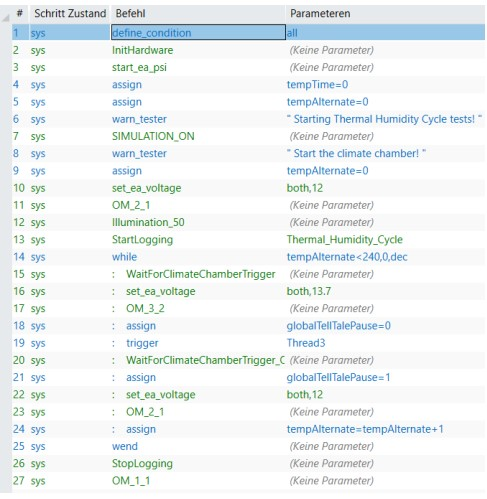
\includegraphics[width= 1\textwidth]{images/CANoe variable system.jpg}
	\caption{CANoe commands list }  
	\label{fig:CANoe commands list}
\end{figure}
\newpage
\subsubsection{Data-logging \& Storage Issues} \label{datalog}

At this point, it is important to introduce the testing procedure enabled by the software setup here called continuous monitoring. 

It is important to be able to provide the customer with measurement records that are uninterrupted over time. When testing DUTs on the basis of functional tests, logging protocols must therefore be used to prove that the assembly behaves according to specification. The keyword here is continuous monitoring. There is no clear definition of this term. If a certain frequency for logging data is specified by the customer, a more detailed analysis of this topic is not necessary, and one can work according to concrete specifications. However, direct numerical specifications for the storage interval of measurement data are often not made in customer specifications. In the following some problems are listed, for which continuous test monitoring can help \cite{ctm}.

\begin{itemize}
    \item Undetected change in environmental conditions
    \item Memory leakage
    \item Intermittent errors due to marginal test designs
    \item Performance degradation due to long-term testing
\end{itemize}

Consequently, in addition to a high measurement frequency to capture the data at all, the logging frequency is also significant. Logging is the automatic creation of a log of software processes. The frequency of logging is a directly related to the type of test and it's definition. For a test that takes only a few minutes, this frequency can be kept high and, for example, a data record can be recorded every second. The memory requirement is then kept within limits. If it is a long-running test with a duration of several hundred hours with unchanging environmental conditions, a successive reduction of the logging frequency is possible. At this point it should be noted that the diagnosis of possible errors and measurement deviations has top priority and an error control function must be ensured during a test. If a limit violation occurs, it must be possible to return to the original logging frequency.


An example of an environmental test with a large total test duration is the High Temperature Operating Endurance (HTOE) test. These tests are defined in CES's internal test definition documents known as QPP or Qualification Program Plan. The QPP is derived from various automotive test specific standards and regulations along with customer requirements. The HTOE test simulates failure modes and the cumulative damage that results from bias operation at different temperatures such as solder plastic creep, crack propagation in many materials, drying of electrolytic capacitors etc. \cite{qpp}. The temperature profile of the HTOE test as a function of time is shown in \hyperref[fig:HTOE Test Cycle]{Fig.5}. 

\begin{figure}[H]
	\centering
	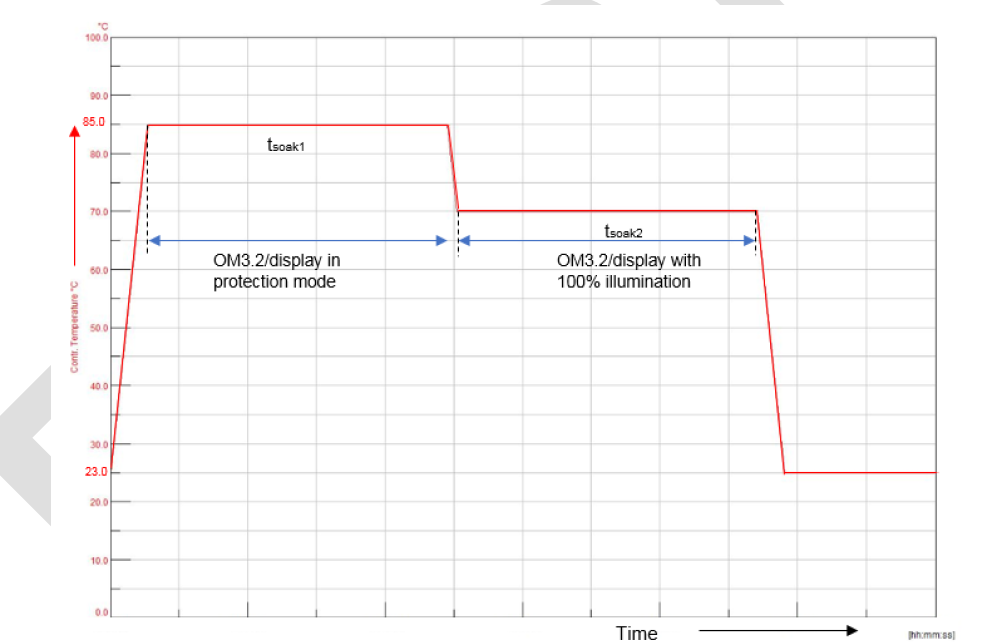
\includegraphics[width= 0.77\textwidth]{images/HTOE.png}
	\caption{HTOE}  
	\label{fig:HTOE Test Cycle}
\end{figure}

Here, for example, longer test times occur where the temperature does not change, such as in the first period when testing at 85° C. This temperature is a test standard and is defined in the AEC (Automotive Electronic Council) Q100 Qualification program for electronic components such as integrated circuits (ICs). The 85° C results from Grade Three of the Ambient Operating Temperature Range, which is defined from -40 to 85° C \cite{aec}. The test is conducted for over 850 hours. If the logging frequency is set at for example, 2 s, we would obtain ~1.5 million data points according to equation below 


\begin{equation}
Datapoints = \frac{Hours * 3600}{Sample Frequency}
\end{equation}

Depending on how the format of logging block is setup in CANoe shown in \hyperref[fig:Measurement Setup]{Figure 3}, each data point could be above 200-250 bytes. This is shown in image below as 'length':

\begin{figure}[H]
	\centering
	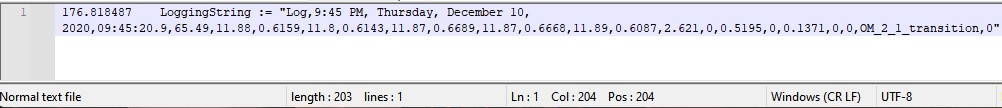
\includegraphics[width= 0.9\textwidth]{images/Datapoint.jpg}
	\caption{Datapoint Size }  
	\label{fig:Datapoint Size}
\end{figure}
 

\begin{equation}
Data Size (in MB ) = \frac{Datapoints * length}{1.048.576}
\end{equation}

So according to the equation above, size of total log from HTOE tests would be around 300-400 MB. There are different types of tests like HTOE defined in QPPs per Qualification round. This would mean that the penultimate size of all data log files per Qualification Test Round would be in multiple Gigabytes. Apart from the data log files shown in fig 2., the CANoe logging setup also generates ".blf" datalogging files. These files are usually in 100s of GB as shown below:

\begin{figure}[h]
  \centering
  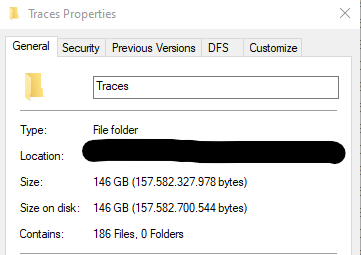
\includegraphics[width= 0.6\textwidth]{images/BLFlocationsize.png}
  \caption{.blf folder}
  \label{fig:Blf File folder}
\end{figure}


\begin{figure}[!h]
  \centering
  
\includegraphics[width= 0.6\textwidth]{images/blfsize.png}
  \caption{.blf file sizes}
  \label{fig:Individual File Size .blf}
\end{figure}

CANoe and CANalyzer support two types of logging formats: message-based and signal-based.
\begin{itemize}
    \item Message-based - 
        A message-based format will store the traffic of bus systems and additional information about the bus communication. In general all bus events (messages) will be logged together with other information like statistics or even disturbances of the bus traffic. These logging files can be easily used for offline analyze of network traffic or for replay on the bus with CANoe.  
    \item Signal-based -
        A signal-based format will store signal values that were extracted from messages transferred over the network. All information about the message itself and additional information about the network and communication will be lost. To log a signal-based file a description (database) for decoding the signal values has to be provided. Signal-based files cannot be directly replayed on the bus but can be easily used for signal analyze in CANoe, CANape or third party tools.
\end{itemize}

ASCII Logging Files (.asc)

\begin{itemize}
    \item Message-based format for reading and writing
    \item Standard ASCII representation
    \item Used for data exchange with third-party programs or to include trace data in documents
    \item Supports messages of all bus systems, system variables, environment variables, internal events, markers and comments
\end{itemize}

Note: ASCII is not recommended at high data rates due to its poorer performance. BLF and MDF format are much better suited for this.

BLF Logging File (.blf) - A .blf file is a binary logging format file created by Vector Informatik CANoe or CANalyzer. It contains a record of the events routed through a car's controller area network (CAN). CANoe and CANalyzer users can review the events a .blf file contains or replay the events on a CAN.


\begin{itemize}
    \item Message-based format for reading and writing
    \item Binary Logging Format (binary format)
    \item Stores the data in binary format in a very efficient way in terms of file size and read/write performance
    \item Supports messages of all bus systems, system variables, environment variables, internal events, markers, and comments
\end{itemize}

BLF is recommended for all new logging \cite{blf}. Hence, all the default logging occurs on CANoe by means of a .blf file which are huge in size. The type of logging file can be set via Logging block in the measurement setup of CANoe described earlier. This thesis will study methods to reduce file size of both log-file types. 

The existing state of implementation of data logging process involves down sampling the logging rate. Down-sampling refers to the process of reducing the number of samples in a digital signal, typically for the purpose of reducing the amount of data that needs to be processed or stored. This can be done by discarding some of the samples, or by averaging multiple samples together. In image processing, down-sampling refers to the process of reducing the number of pixels in an image. This can be done by discarding some of the pixels, or by averaging the values of multiple pixels together. The goal of down-sampling is usually to reduce the computational and storage requirements of an image processing pipeline, while still preserving the important information in the image. According to existing setting, the user can configure the sampling rate before testrun using a GUI created using CANoe \& CAPL. This is demonstrated below : 

\begin{figure}[h]
  \centering
  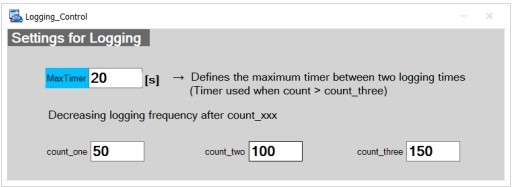
\includegraphics[width= 0.6\textwidth]{images/loggingfreq.jpg}
  \caption{Down-sampling}
  \label{fig:downsampling}
\end{figure}

Upon test setup, using this GUI the user can set the sampling rate. The "Max. Timer" option is used for setting the maximum period of data logging. However, before Max. Timer is implemented the logging process undergoes 3 step calculation, i.e, "count\_one", "count\_two", "count\_three". Initially data logging occurs at a frequency set by the Logging block mentioned earlier. The count steps are counter based flags established to check for invalid data during that particular increment period. Invalid data is determined by values that are outside the tolerance ranges defined for the test. As shown in figure, during increment, data will be monitored based on default data log frequency until 50 counts, if no error occurs till 50 counts, the average value of 50 data points is logged into the system. Thereafter counter is incremented to count\_two and then similarly after 100 non error increments, the averaged value of 100 data points is logged and then similarly for count\_three. If count\_three also provides error free data monitoring, then the data logging period is set to 20 s. Thereafter, the 
data logged is an average of values in the period of Max. Timer. The averaging is also influenced by a counter defined pre-test run "AvgNoofMeas". Towards, the end a reduced data log file is generated that is substantially down-sampled yet large in size. The thesis is focused on finding a possible alternative to this approach with primary focus on achieving maximum compression without loss of data. 
%-------------------------------------------------------------------------------------------------------------------------------------------------------------
\begin{comment}
\subsection{Research direction 2} \label{sec:rw_dir2}
\cite{wintersberger} befasst sich mit einer umfassenden und klar definierten Taxonomie der zwei Hautprozesse ``handover'' und ``handback''. Er kommt zu folgender Schlussfolgerung:

\begin{itemize}
	\item[1.] Handover - von der automatisierten zur manuellen Fahrt			  
	\item[2.] Handback - von der manuellen zur automatisierten Fahrt			  
\end{itemize}


\subsubsection{Relevanz für die eigene Arbeit - Direction 2}

Lorem ipsum Lorem ipsum.


\subsection{Schlussfolgerung}
Zusammenfassung des Kapitels, Ableitung von Empfehlungen, etc. für die eigene Arbeit.

\begin{itemize}
	\item Lorem ipsum \autoref{sec:hardware}.
	\item Lorem ipsum lorum ipsum \autoref{sec:hardware}.
	\item Lorem ipsum \autoref{sec:rw_dir2}.
	\item ...
	\item Lorem ipsum lorem ipsum lorem ipsum\autoref{sec:rw_dir2}.
\end{itemize}
\end{comment}			% 2. Literaturanalyse/Related work analysis
\newpage
\iffalse
\thispagestyle{myPageStyle}
\section{Requirements and Goal Definition}\label{sec:Requirements}
Before discussing and describing the concepts and findings in details for this study, it is important to define the goals. Without a definition and a description of goals, system development is more difficult to implement. Requirements Engineering comes to role at this stage. After the technology concepts have been explained on the basis of these requirements, the final concept is selected on the basis of various evaluation criteria, which are themselves ranked according to importance.

\subsection{Introduction to Requirements Engineering}
In this thesis, we deal with development of algorithms and software. Hence, it is essential to understand the methods which are industry standards for developing software. SDLC stands for Software Development Life Cycle. It is a process that defines the steps or phases that a software development project goes through from the initial planning stages to the final implementation and maintenance of the software.

The SDLC process is usually divided into several phases, which may vary depending on the specific method used, but commonly include:

\begin{itemize}
    \item Requirements gathering and analysis: This phase involves understanding the needs of the users and stakeholders, and identifying the functional and non-functional requirements of the software.
    \item Design: This phase involves creating a detailed design of the software, including the system architecture and user interface.
    \item Implementation or coding: This phase involves writing the code for the software based on the design.
    \item Testing: This phase involves testing the software to ensure that it meets the requirements and is free of bugs.
    \item Deployment: This phase involves installing the software on the target system and making it available for use.
\end{itemize}

The SDLC process helps to ensure that the software is developed in a structured and organized way, and that the final product meets the needs of the users and stakeholders. Different SDLC models such as Waterfall, Agile, V-Model, Spiral Model, etc can be used depending on the needs of the project and the organization.

V Model, Waterfall, and similar methods are all traditional SDLC models that are often used in requirement engineering. The V Model is a software development process that follows a linear and sequential approach, with each phase of the process flowing in a V-shape from the requirements phase to the testing phase. The model is based on the idea of "verification and validation", where the requirements are verified during the design phase, and the system is validated during the testing phase.These methods are commonly used to plan, design, and build a product. They are not part of Requirements Engineering but they rely on requirement engineering as the first phase. The Requirements Engineering phase is where the requirements are gathered, analyzed, and specified before the design and development of the product begins.

Of all the methods mentioned, below is a brief explanation of one of the most used SDLC model before discussing requirements engineering :
V-Modell is a German software development process model that is widely used in Germany and other German-speaking countries. It is a phased, linear, and sequential model that is often used in government and defense projects. The model is based on the idea of "verification and validation" where the requirements are verified during the design phase, and the system is validated during the testing phase.

The V-Modell is divided into four main phases:
\begin{itemize}
    \item Planning and Organization: This phase involves defining the project goals, outlining the project plan, and identifying the project team.
    \item Analysis and Concept: In this phase, the requirements are gathered, analyzed, and specified. This includes defining the system architecture, and creating a detailed project plan.
    \item Realization: This phase involves the design, development, and implementation of the system. This includes the coding, testing, and integration of the system.
    \item Deployment and Maintenance: This phase involves the deployment of the system, the training of users, and the maintenance of the system.
\end{itemize}

The V-Modell also includes several intermediate phases such as the "System Design" and "System Test" phases. These phases are focused on verifying and validating the requirements at different stages of the development process. The V-Modell also includes specific guidelines for documentation, quality assurance, and project management.

\begin{figure}[!h]
    	\centering
    	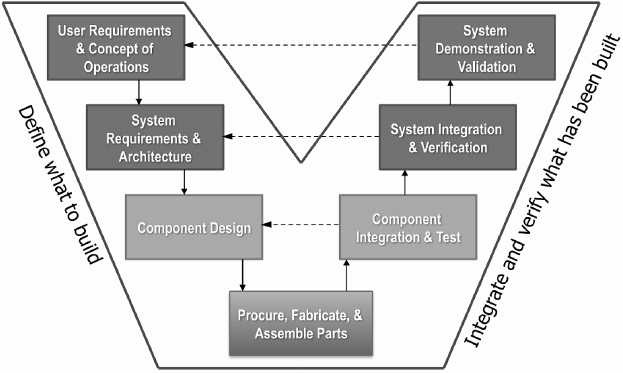
\includegraphics[width= 0.85\textwidth]{images/Typical-systems-engineering-V-model.png}
    	\caption [V-Modell]{V-Modell Diagram \protect\cite{vmodel}}  
    	\label{fig:V-Modell}
\end{figure}

One of the main advantages of the V-Modell is its focus on the verification and validation of requirements. This helps to ensure that the end product meets the needs of the customer, while also taking into account safety, performance, and other critical factors. However, the V-Modell can be inflexible and may not be suitable for rapidly changing environments where the requirements may evolve over time.
The first step of this approach is to make a list of requirements and define them. In the table given below, a list of requirements with their brief definition is provided. Additionally, the type of requirement is also mentioned. 


Every project will have certain requirements that are defined to be Must-Have (MH). It is imperative that these requirements are met in order to deem the project successfully completed. These requirements are called MVP or Minimum Viable Product. MVP is a concept that is often used in product development and management. It refers to the version of a product that has just enough features to be able to be released to a limited group of customers (often called "early adopters") and gather feedback. The idea is to validate the product's value proposition and gather feedback before investing more resources into development. MVPs are often used in the context of lean startup methodologies, which prioritize learning and validation over the pursuit of a perfect product. So MVP is a concept that can be used in product management but it is not a part of product management. Once the MVP has been created one would always want to have more features added to the tool/program for enhanced sophistication. Such features are part of the requirements which are defined as Nice-to-have (NTH) requirements. These requirements can include things like additional convenience features, aesthetics, or performance improvements. They are not essential for the core functionality of the product, but they can add value and make the product more attractive to customers.

\begin{table}[h]
    \centering
    \begin{tabular}{ |p{4cm}||p{4cm}||p{4cm}|}
     \hline
     \textbf{Requirements} & \textbf{Description} & \textbf{Type of Requirement} \\
     \hline
     Compression Factor & Achievable compression without loss of data  & MH\\
     \hline
     User Friendly & Ease of access for end-user & MH  \\
     \hline
     Data Evaluation Capability & Capability to evaluate and utilize compressed data for additional purposes & MH  \\
     \hline
     Troubleshooting Friendly & End-user must be able to troubleshoot algorithm/program errors with ease & MH  \\
     \hline
     Multi-format program & The compression should be applicable to as many file types as possible & NTH \\
     \hline
     Extensibility & Possibility to modify the algorithm/program for additional features in future & NTH \\
     \hline
     Data Re-usability & Encryption and Decryption of compressed data should be possible, if applicable & NTH\\
     \hline
     Data Evaluation  & Capability to utilize compressed data and perform data evaluation as desired & MTH \\
     \hline
    \end{tabular}
    \caption{List of Requirements}
    \label{tab:Requirements List}
\end{table}

\clearpage



		  % 3. Implementation, Technical Setting, Prototype
\newpage

\thispagestyle{myPageStyle}
% Kapitel 8 - Diskussion
%\clearpage
\section{QFD \& Algorithm Selection}\label{sec:Algorithm definition}

This thesis studies different approaches to develop the algorithm to achieve data reduction. In this chapter different approaches to achieve data compression would be analysed. Also, QFD is a useful tool to define and analyse the requirements and consequently derive an appropriate solution to the problem in the form of an algorithm. The following sub-chapters discuss different approaches to achieve data reduction along with methods like pairwise comparison and weighted analysis used to determine the most optimal approach of all.

\subsection{Mathematical Reduction}
%\ref{datalog}
As mentioned in previous chapters, the existing implementation is focused primarily on the down-sampling of data-stream. Thereafter, the average of each sample is calculated and then stored. While this is not a broken approach, there is a good amount of room for improvement here. While down-sampling with active monitoring for error free sample is a good approach, the existing method has a multi-step approach to achieving the down-sampling and then averaging the results. This approach would be computationally demanding than regular data log generation, as it undergoes a 3 step monitoring process before settling down on the pre-selected sampling frequency to down-sample the data-stream. This would require relatively more time also, naturally, than simple data-log generation. 

Since the logs consists of numerical values, primarily, mathematical approaches for reducing the size of data can definitely not be ignored or discarded. Statistical methods like mean, median, standard deviation or variance could be utilized here since all of them deal with condensing chunks of data into singular or smaller meaningful arithmetic numerals. A quick explanation and summarising of different statistical approaches is hence needed. 

The first method of mean is of particular interest here. The method of mean involves in finding the averages of values and condensing a larger set of value into singular or smaller sets of data that indicate the central tendency. There are several kinds of mean in mathematics, especially in statistics. Each mean serves to summarize a given group of data, often to better understand the overall value (magnitude and sign) of a given data set. For a data set, the arithmetic mean, also known as "arithmetic average", is a measure of central tendency of a finite set of numbers: specifically, the sum of the values divided by the number of values. The arithmetic mean of a set of numbers x1, x2, ..., xn is typically denoted using an overhead bar, $\bar{x}$. \cite{mean} 

There are primarily three types of means that are generally used in statistics. They are as follows: 

\begin{itemize}
    \item Arithmetic Mean
    \item Geometric Mean
    \item Harmonic Mean
\end{itemize}

\textbf{Arithmetic Mean} : also known as the average, is a statistical measure that is used to determine the central tendency of a set of numerical data. The arithmetic mean is calculated by summing all of the values in a data-set and dividing the total by the number of values in the data-set. The arithmetic mean is commonly used in many different fields and is one of the most widely used statistical measures. It is particularly useful in situations where the distribution of data is symmetric and the data is not skewed. It is easy to calculate, easy to understand and is useful in many different types of analyses.  One of the main advantages is that it is easy to understand and calculate. Because the arithmetic mean is based on the sum of all values in a data-set and the number of values in the data-set, it is easy to compute and understand the results. However, there are also some limitations to using the arithmetic mean. One of the main cons is that it can be affected by outliers or extreme values in the data-set. For example, if there is a single extremely large value in a data-set, it can skew the overall mean and make it unrepresentative of the majority of the data. Additionally, the arithmetic mean is not useful for data-sets with skewed distributions, such as those with a lot of small values and a few large values.

The below equation shows how arithmetic mean is calculated : 

\begin{equation}
\bar{x} = \frac{x1 + x2 + x3 + ... + xn}{n}\
\end{equation}

\textbf{Geometric mean} :   is a measure of central tendency that is used to find the average value of a set of numbers by multiplying them together and taking the nth root, where n is the number of numbers in the set. It is often used when working with data sets that have skewed distributions, such as when dealing with exponential growth or decay. One of the main areas of implementation for the geometric mean is in finance and economics, where it is used to calculate the average rate of return on an investment over a period of time. This is particularly useful when comparing investments with different volatility levels, as it gives a more accurate picture of the overall performance of the investment. The geometric mean has some advantages over other measures of central tendency such as the arithmetic mean. It is less sensitive to outliers and extreme values, which makes it a better measure of central tendency when working with skewed data. However, the geometric mean also has some downsides, such as it is not defined for negative values, and it is also not defined for data-sets that contain zero or negative numbers. 

Additionally, it can be difficult to interpret the geometric mean when working with large numbers, as it can be difficult to understand the meaning of the nth root of a large product. In conclusion, the geometric mean is a useful measure of central tendency that is particularly well-suited for data sets that have skewed distributions, and is widely used in finance and economics, statistics and research, it may be not appropriate for data-sets containing negative numbers and it can be difficult to interpret large values. Geometric mean is represented as below :

\begin{equation}
    \left(\prod _{i=1}^{n}x_{i}\right)^{\frac {1}{n}}={\sqrt[{n}]{x_{1}x_{2}\cdots x_{n}}}
\end{equation}


\textbf{Harmonic Mean} :  a type of average that is commonly used to calculate the average of rates or ratios. It is calculated by taking the reciprocal of the arithmetic mean of the reciprocals of the given numbers. The purpose of the harmonic mean is to provide a fair representation of the average when the values being averaged have varying degrees of impact or importance. For example, when calculating average speed, harmonic mean is preferred over arithmetic mean as it gives more weight to the lower speeds. One of the major advantages of the harmonic mean is that it is not affected by outliers and extreme values, making it a more robust measure of central tendency. However, the harmonic mean cannot be calculated if any of the values in the set are zero or negative. This is a major disadvantage as it can lead to undefined or meaningless results. In general, harmonic mean should be used when the data set contains rates and ratios and when the values are not skewed by outliers. In cases where the data contains only positive values, and that the large values does not skew the data, then harmonic mean is an appropriate measure of central tendency. The formula for harmonic mean is :

\begin{equation}
    HM = \frac{n}{1/x1 + 1/x2 + ... + 1/xn}
\end{equation}

From the above descriptions, each of the methods seems to be useful in their own way. With varying and widely skewed data, Geometric mean and harmonic mean seem to be able to deal with in a much better way than arithmetic mean. However, arithmetic mean is robust and practically suitable over the other two methods when it comes to deal with signed numbers, i.e positive , negative or zeros. While geometric mean and harmonic mean are well suited for a varied range of data, it is important to understand that this thesis studies a specific set of data-logs and logging processes. The data-sets involved in here deal with parameters such as voltage and current of the DUTs. This means if the DUTs are operated in any mode which doesn't draw power, i.e regenerative mode or non-linear mode there is a possibility of negative values of voltage and current. There are also scenarios defined in QPP where the device is in sleep mode, i.e. voltage and current values are zero. Considering the factor of area of deployment, arithmetic mean appears to be the most suitable option.

However, we are dealing with huge amount of data-sets and they are captured in real-time. The testing of DUTs are done to verify and validate that they function in accordance to the requirements of the customers. During the development phase, the performance of the DUT is defined. However, these LTT are necessary to validate the adherence to the development phase and thus even-though it is possible to define the expected output, it is not certain how close the real output would be to the expected. If the DUT has zero faults and functions according to definitions, the expected and real output must be same. However, there is always difference between theory and practical execution of any processes. Thus, it is highly probable that the output differs from the expected output or the distribution of the data is highly skewed. This indicates that even arithmetic mean would be unable to deal with the data-sets because of it's inability to maintaining central tendency of the data-sets in the event of skewed data-sets. The arithmetic mean would eventually sway in the direction of the deviation of the data-set thus losing the central tendency of the data-set or conveying a meaningful summary of the total data-set. One method that could help overcome this problem is filtering.

Data filtering is the process of selecting a subset of data from a larger data-set based on certain criteria. There are several different methods that can be used to filter data, including:

\begin{itemize}
    \item Removing outliers: This method involves identifying and removing data points that are significantly different from the rest of the data set. This can be done using statistical techniques such as the Z-score method or the Interquartile Range (IQR) method.

    \item Clipping: This method involves setting a lower and upper limit on the data values and removing any data points that fall outside of this range. This can be useful in cases where there are extreme values that do not represent the typical behavior of the data set.

    \item Binning: This method involves grouping data points into a smaller number of "bins" based on a specific criteria. This can be used to remove noise from the data by grouping similar data points together.

    \item Smoothing: This method involves applying a mathematical function to the data set in order to reduce the amount of variation in the data. This can be useful in cases where there is a lot of noise in the data.

    \item Interpolation: This method involves estimating missing data points based on the values of the surrounding data. This can be useful in cases where there are missing data points that need to be filled in.

    \item Data imputation: This method involves replacing missing values in the data-set with some statistical estimate of the missing values. This can be done by using techniques like mean, median and mode imputation.

\end{itemize}
\newpage

For the type of data-sets studied in this thesis, removal of outliers and clipping seem to be suitable approaches for data filtering. 

Removal of outliers is the simplest type of data filtering. Even though sometimes outliers should be kept in the data set as part of the analysis, such as in the case of modeling of credit risk, fraud, and other rare events, in most of the cases, they represent unnecessary information and should be removed. Unnecessary outliers are noise in the data and mostly can reduce the predictability of the model \cite{filter}. The Z-score method, also known as the standard score method, is a statistical method used to identify outliers in a data-set. It is based on the idea of measuring the number of standard deviations a particular data point is from the mean of the data-set. A Z-score of less than -3 or greater than 3 is generally considered an outlier. The IQR (interquartile range) method is another statistical method used to identify outliers in a data-set. It is based on the difference between the third and first quartiles of the data-set. A data point is considered an outlier if it is more than 1.5 times the IQR below the first quartile or above the third quartile.

Both of these methods are based on the assumption that the data follows a normal distribution. Normal distribution, also known as the Gaussian distribution or bell curve, is a probability distribution that describes how frequently a certain set of data occurs. It is defined by its mean (average) and standard deviation (a measure of how widely the data is spread out). The distribution is symmetric around the mean, and the probability of observing a data point is highest at the mean, and decreases as the data point moves further away from the mean. The standard normal distribution, which has a mean of 0 and a standard deviation of 1, is a particularly important case of the normal distribution that is used in many areas of statistics and probability theory. In a normal distribution, about 68\% of the data falls within one standard deviation of the mean, about 95\% falls within two standard deviations of the mean, and about 99.7\% falls within three standard deviations of the mean. They are simple and easy to use, but may not be appropriate for data-sets that do not follow a normal distribution.

\begin{figure}[!h]
    	\centering
    	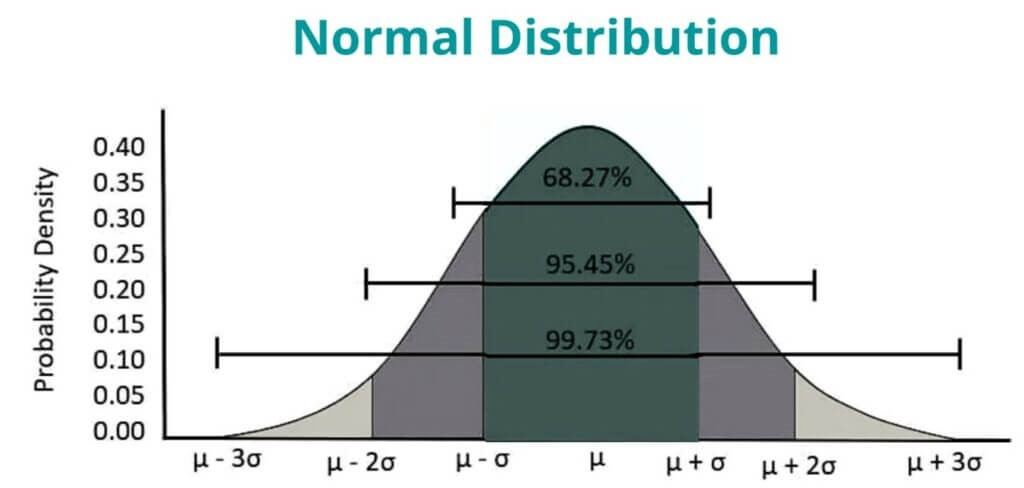
\includegraphics[width= 0.9\textwidth]{images/Normal-Distribution-1-1024x556.jpg}
    	\caption [Normal Distribution]{Normal Distribution \protect\cite{Normal}}  
    	\label{fig:Guassian Distribution}
\end{figure}


In data science, clipping refers to the process of limiting the range of values in a data-set. This is typically done to remove outliers or to handle cases where the data has extreme values that may skew the results of an analysis. Clipping can be applied to both uni-variate (single variable) and multivariate (multiple variable) data-sets. The process of clipping involves setting a threshold, and any data points that fall outside of that threshold are replaced with the threshold value. This can be done by replacing all values below a certain minimum threshold with the minimum threshold value, and all values above a certain maximum threshold with the maximum threshold value. Clipping can be useful in situations where extreme values in the data can have a disproportionate impact on the results of an analysis, such as in statistical modeling or machine learning. It can also be used as a pre-processing step to improve the performance of algorithms that are sensitive to outliers. 

Compared to the Z-score or IQR method for removing outliers the clipping method appears to be more appropriate for the data-sets dealt with in this thesis. The values or parameters monitored in the LTT are usually defined by tolerance limits. These tolerance limits are defined in each QPP documents. Every electronic device has a tolerance range for it's operation. When the device operates under the tolerance range, upper tolerance and lower tolerance limits, the device is considered to be functional and the data from the device is considered valid. With passage of time the components in DUT will end up having wear \& tear due to constant exposure to varying levels of external factors like temperature, shock etc as well as changing modes of operations. These deterioration means there would be change in output values that will not lie in the desired tolerance ranges. This is called as drift and would also be discussed in the next chapter. 

Clipping is a good approach to analyse the data as it permits only values or data lying in the tolerance window. The data that lies inside this window is valid and hence suitable for arithmetical operations such as arithmetic mean. The clipping method can also be used as means to observe the drift. The drift could be observed in the way, where the no. of values the end up lying outside of the tolerance windows can be observed and then determined whether the device is undergoing aging or deterioration or not. 

Thus, a combination of clipping and arithmetic mean can thus help in reducing the data size as well as making the condensed data more meaningful for the end user to analyze. 
\newpage

\subsection{Compression Algorithms}

Data, in general, could mean any type of output. Anything ranging from images to texts, videos to signals, numbers to e-mails can be called as Data. With increase in development of technology in different domains, the quality of data has improved significantly. At the same time, the size of data has also increased proportionately. With this trend arose the demand to efficiently store data. For this purpose, several data compression techniques have been developed in various fields over the years. Data compression algorithms are methods used to reduce the size of data without losing important information. 

There are several types of data compression techniques that are in existence. Of those, here are some common and relevant types of techniques : 

\begin{itemize}


    \item \textbf{Lossless compression} : These algorithms are designed to compress data in such a way that the original data can be exactly reconstructed from the compressed data. Examples of lossless compression algorithms include:
    \begin{itemize}
        \item LZW
        \item Huffman coding
        \item Run-length encoding
        \item Arithmetic Encoding
    \end{itemize} 


    \item \textbf{Lossy compression} : These algorithms are designed to compress data by discarding some of the information that is considered less important. These algorithms are most commonly used in image and audio compression. Examples of lossy compression algorithms include:
    \begin{itemize}
        \item Discrete Cosine Transform (DCT)
        \item Fractal compression
        \item Transform coding
        \item Quantization
    \end{itemize} 

    
    \item \textbf{Dictionary-based compression}: These algorithms are based on the idea of replacing a sequence of data with a reference to a dictionary of common sequences.
    Some examples of the same are :
    \begin{itemize}
        \item LZ77
        \item LZ78
        \item LZW
        \item LZMA
    \end{itemize} 
    
\end{itemize}

Lossless compression is a method of compressing data in such a way that the original data can be recovered exactly from the compressed data, without any loss of information. Lossless compression is used in situations where it is important to maintain the integrity of the original data, such as in medical imaging, scientific data, and text documents. The most common lossless compression algorithms are based on statistical methods, such as Huffman coding and arithmetic coding, which use the frequency of occurrence of different symbols in the data to create a more efficient representation of the data. Run-length encoding (RLE) is a method of data compression that is used to represent a sequence of data where repeating values are replaced with a single value and a count. The basic idea behind RLE is to identify runs of repeating values, and represent them using a shorter notation. For example, if we have a sequence of data consisting of the values 1, 1, 1, 2, 2, 3, 3, 3, 3, we can represent this using RLE as "3x1, 2x2, 4x3". This method is commonly used for image compression, as it is effective for image data that contains large areas of solid color. For example, a large image of a blue sky would contain many pixels with the value of blue, and RLE can efficiently compress this data. Lossless data compression algorithms can be used to compress text, images, audio and video files. They are also used in file archiving, backups, and data storage.


Lossy compression is a method of data compression in which some of the original data is discarded in order to achieve a higher level of compression. The goal of lossy compression is to retain the most important information while discarding less important information. This type of compression is commonly used in image and audio compression, as well as in video compression. One of the most widely used examples of lossy compression is JPEG, which is used for compressing images. In JPEG, the image is divided into small blocks called macro-blocks and each block is transformed into the frequency domain using the Discrete Cosine Transform (DCT). The DCT coefficients are then quantized and encoded using Huffman coding, which discards the less important coefficients. This results in a smaller file size but with a loss of some of the original image information.In addition, video compression like h.264 and h.265 also use lossy compression technique to compress the video data, they will take advantage of the temporal and spatial correlation of video to remove the redundant data and keep the important information. Lossy compression is widely used in applications where storage space is limited, such as in mobile devices and in streaming media. 

Dictionary-based compression is a method of data compression that utilizes a predefined dictionary of words or phrases to compress a given input stream of data. The basic idea behind this method is that many natural language texts, as well as other types of data streams, contain repeating patterns or sequences of characters, which can be replaced by shorter codes that represent those patterns in the dictionary. One of the most well-known examples of dictionary-based compression is the Lempel-Ziv-Welch (LZW) algorithm, which is commonly used to compress text files, image files, and other types of data. The LZW algorithm works by building a dictionary of phrases that are encountered in the input data, and then replacing each phrase with a code that corresponds to its position in the dictionary. Another example of dictionary-based compression is the Burrows-Wheeler transform (BWT), which is used in the bzip2 and gzip compression utilities. BWT is used in the bzip2 and gzip compression utilities, which are commonly used to compress log files, text files, and other types of data. 

From the above descriptions, it is very clear that lossy compression is not a suitable approach for compression of the data-sets. Each sampled data-point is important in the sense that regardless of valid or invalid data, it is an indication of the state of DUT. The valid data-points could be compressed or condensed into smaller sets of data-points while the invalid data-points can be used to study the characteristics of the errors in the DUT. Using lossy compression could cause loss of data-points which could change the complete characteristic of the log-file or analysis performed by the end user. 
%\ref{datalog}
Dictionary-based compression from it's characteristics is a subset of lossless compression. However,the target area for dictionary-based compression is different to the data-sets being utilized in this thesis. Going back to chapter 2, there are two different types of log files that are generated by the test systems, i.e .blf files and .asc files. Dictionary based compression use file zipping as one of the methods for data compression. Since .blf files are files that are 100s of GB in size and consist of different types of data-sets, file zipping appears to be a possible solution. The .blf files contain different types of data related to CAN traffic and metadata about that traffic. Hence, it is a possibility that one single custom algorithm could not be implemented on .blf files and it might require different approaches. File zip is a plausible solution for reducing such complexity and hence worth consideration. 

Lossless compression is the technique that is of most interest in this study. As mentioned earlier, a compression technique that could achieve data reduction without loss of information in crucial to handle the data-sets studied in this thesis. Of all the compression techniques which achieve lossless compression, RLE Encoding or Run-length Encoding is a method that can achieve such a lossless compression. It encodes runs of repeated data elements into a single data elements and a count. The method works by scanning the input data and counting the number of consecutive occurrences of each data element. These counts are then encoded along with the data element in the compressed data stream. An example of the same has been already discussed above.     

The RLE encoding can be used for dealing with .asc files. The .asc files are also log files generated from test-systems like .blf files. However, instead of consisting of information of all types of data from the test system like .blf files, the .asc files are parameter based log files. They contain information about parameters like voltage, current, time, temperature etc. in them. Since, the files contain multiple sets of similar data, RLE encoding can be considered a feasible solution to compress files of such types. 

\newpage

\subsection{Processing}

Having understood possible methods to reduce the file size to achieve meaningful data compression, it is necessary to understand the type of processing that could occur on the these data-sets. Processing is an important aspect of handling the log files as it deals with fetching , segregating and compressing the data. There are two types of data processing methods that can be implemented on the test systems. 

1) \textbf{Real-time Processing}: It is a method of data processing where data is processed immediately as it is generated or received. This method is used in applications that require immediate processing, storage, and retrieval of data, such as financial transactions, stock trading, and medical equipment monitoring. Real-time processing is more complex than batch processing, as it requires the immediate processing and storage of data, as well as the ability to retrieve data quickly. The main advantage of real-time processing is that it provides prompt and up-to-date information, which is crucial in many time-sensitive applications.

As is known already, the test systems are controlled by CANoe. This means that data logs can be processed at source or at destination. 

The data-logs are generated from the logging blocks defined in CANoe and written in CAPL code. Real time processing in this context would mean that logging blocks be used as source and compression algorithm be written in CANoe using CAPL code for the data-logs. System variables play crucial role in real time processing because data is read and written onto them from the test systems. If a buffer system is created, then it is possible read and write data that is logged from the test system into the compression algorithm simultaneously. A buffer is a temporary storage area in computer memory that holds data waiting to be processed or data that has been processed but not yet stored in its final destination. Buffers play an important role in computer systems by allowing the smooth flow of data between different stages of processing, reducing the impact of differences in data processing rates, and ensuring that data is properly managed and protected during transfer. There are different types of buffers, including input buffers, output buffers, and data buffers, that serve different purposes depending on the system architecture and the type of data being processed. Some of the types of buffers that could be considered useful for this purpose are as follows:

\begin{itemize}
    \item \textbf{FIFO} : FIFO buffer operates like a queue where the oldest data is processed first and new data is added at the end. It's advantages include ease of use and simplicity in processing data, as well as being well-suited for real-time applications. However, it requires larger memory space and is less efficient for data manipulation operations.

    \item \textbf{Circular Buffer} : Circular buffer operates in a cyclic manner where the oldest data is overwritten when the buffer is full. It's advantages include efficient use of memory and well-suited for real-time applications. It's main disadvantage is the complexity of implementation.
\end{itemize}

A circular buffer, also known as a ring buffer, is a data structure that is commonly used in real-time systems for buffering data streams. It is implemented as an array that has a fixed size, and a read and write pointer. When the write pointer reaches the end of the array, it wraps around to the start of the array. This is a much more memory efficient approach to process the data in real time compared to the FIFO buffer approach. FIFO even though being a simpler approach of implementation, is a resource heavy approach since it waits for the complete buffer to be written, filled and old discarded before the new data could start writing into it. 

These buffer systems could be defined inside a CAPL code which fetches data from the logging block with help of system and environmental variables. This would ensure that the logging and compression occurs simultaneously. With the help of buffers, data from the sensors could be read in real-time, then filtered for validity and then passed on to final logging block. The result of this complete process would be a log file in .asc format for the user to analyse in the most compressed form. The advantage to this approach is that no temporary storage for log files is required on external computers. Test-systems or systems running CANoe should have necessary computing memory available to facilitate this since it's a real time resource heavy task.


2) \textbf{Batch Processing} : It is a method of data processing where data is accumulated over time and processed in a single group or batch. This method is commonly used for routine tasks such as billing, and accounting. The main advantage of batch processing is that it can handle large amounts of data efficiently, as all the data is processed at once. Another advantage is that it allows for better use of resources such as processing power and memory. However, batch processing can also be time-consuming, as data must be accumulated before it can be processed, and the processing time may be lengthy, especially for large amounts of data. It is more suitable for routine tasks that do not require immediate processing and retrieval of data. 

The batch processing method gives opportunity to use different tools to analyse the log-files and process them. The log files in the .asc \& .blf format are stored in the test laptops at the end of LTT. The .asc files can be opened by default on CANoe as well as external programs like MS Excel unlike .blf files which can be accessed exclusively using CANoe. Batch processing of .asc format files is hence possible using programs like MS Excel. Although .asc aren't natively supported by MS Excel, it is possible to open, read and edit them in MS Excel using MS Excel wizard. The wizard allows to set the format of the file which is quite similar in approach to reading a .csv file in excel and thus enables to read the .asc file in user readable format. Excel Macros are then used to set filters, highlight specific data and many other purposes for the test engineer to analyse the log files and understand the performance of the DUTs. It is possible to write a VBA script that would compress the corresponding by filtering, segregating, summarizing the datas in the log files and then saving the compressed file. 

Another approach is to use a software tool or language to perform the data compression on the stored .asc files. Python is a very promising tool that could help in achieving this goal. Python has various libraries that enable it interact with files of various data types. This is of primary importance because to process the files, it is important to be able to read and write on them. Apart from this feature, python has many in-built mathematical functions pre-defined such as mean, variance etc. Python is also a very handy tool in dealing with MS-Excel files of .xls* formats. This is also crucial as python could be utilised as a method to convert .asc files into easy to access .xls* format files after performing data compression. Since python is a very robust and user-friendly tool, it is also possible to perform various types of analysis on the final log data or compressed data if ever needed by the engineer. 
\newpage
\subsection{QFD}

Quality Function Deployment (QFD) is a comprehensive approach to product development that involves a team of stakeholders working together to identify customer needs and create a product or service that meets or exceeds those requirements. It is a customer-focused methodology that aims to ensure customer satisfaction by designing a product or service that addresses customer needs and wants. One of the key advantages of QFD is that it helps to ensure that customer needs are understood and addressed early in the product development process. By involving customers and other stakeholders in the design process, QFD helps to ensure that the final product meets their needs and expectations. Additionally, QFD helps to improve the product development process by identifying areas where improvements are needed and by evaluating the trade-offs between different options or alternatives.

QFD is often used in manufacturing, service, and healthcare industries. It can be used for developing new products or services, as well as for improving existing ones. It is also used in quality management and process improvement. A short example of QFD in action is a car manufacturing company that wants to improve customer satisfaction with their vehicles. In this case, the car company would use QFD to gather customer feedback and identify customer requirements, such as fuel efficiency, safety features, and comfort. Next, they would use QFD to develop product characteristics, such as engine size and weight, and evaluate trade-offs between different options or alternatives. Finally, they would use this information to improve their existing vehicles and develop new ones that meet or exceed customer requirements.

QFD differs from similar approaches in that it is a customer-focused methodology that aims to ensure customer satisfaction by designing a product or service that addresses customer needs and wants. Additionally, QFD is a comprehensive approach that involves multiple stages, including the identification of customer needs, the development of product characteristics, and the evaluation of trade-offs between different options or alternatives.

There are five different approaches that can be derived from the study of different methods for compression from the sub-chapters above. These are as follows : 

\begin{itemize}
    \item Data compression via mathematical reduction in real-time processing : The algorithm is implemented on CANoe platform with the clipping and arithmetic mean to reduce the size of final log data.

    \item Data compression via mathematical reduction in batch processing : The algorithm is implemented via Python as post processing method with clipping and arithmetic mean to reduce the size of existing logged data.

    \item Data compression via byte size reduction in real-time processing : Run Length Encoding algorithm is implemented on CANoe to reduce the size of the log file.

    \item Data compression via byte size reduction in batch processing : Run Length Encoding algorithm is implemented on existing log files via Python.

    \item Data compression via mathematical reduction through a combination of real-time and batch processing : This is a combination of two processing methods so that reduction can be processed in real-time on CANoe system and then using the python to perform analysis on the reduced data
\end{itemize}


\subsubsection{Pairwise comparison \& Weighted Analysis} 

Pairwise Comparison is a decision-making technique used to compare and rank items based on their relative importance, priority or weight. It is a systematic method that is used in several fields such as software engineering, project management, operations research and decision theory. The aim of pairwise comparison is to determine which of two items is preferred or considered more important, or to rank a set of items in order of importance.

In pairwise comparison, each item is compared with every other item, and the results are recorded in a matrix. This matrix is used to compute the relative importance of each item. Pairwise comparison is used to quantify the relative strength of relationships between two items, which can then be used to rank them. For example, in software engineering, pairwise comparison can be used to rank requirements, in order to determine which ones are most important and should receive priority in development.

One of the advantages of pairwise comparison is that it provides a simple and systematic way to rank items, and it can be used to compare items with different attributes. The approach is highly flexible and can be adapted to a variety of decision-making situations. It is particularly useful when there is no clear objective method of comparison, or when the items being compared are subjective in nature.

Another advantage is that pairwise comparison is easy to understand and can be performed by people with a wide range of knowledge and expertise. It is also less time-consuming and less expensive than other methods, such as multi-attribute decision-making methods, which require more data collection and analysis.

Before performing pairwise comparison it is important to list the requirements that are analysed by this method : 

\begin{itemize}
    \item Compression factor 
    \item User friendliness  
    \item Data evaluation capability 
    \item Troubleshooting friendly 
    \item Multi-format support 
    \item Extensibility  
    \item Data re-usability 
    \item Additional resources
    \item Execution time
\end{itemize}

This thesis studies two types of log files : .asc and .blf files. For the .asc files there are multiple options for achieving data compression since .asc file is not platform restricted. It is possible to access .asc files even without CANoe software. Moreover, they are configurable log file in the sense, it can be set via CANoe - CAPL what parameters should be logged into .asc files. Since the type of data occurring in a .asc file is already and the file is always open for access it is possible to perform data compression on these files using different approaches. 

However, the same cannot be said in the case of .blf files. The .blf file are inaccessible without CANoe platform. This makes it inaccessible to 3 out of 5 data compression methods discussed above which include both the batch processing methods and the third method being the combination of real-time and batch processing method. This leaves the .blf files to be compressed by remaining methods of real-time processing : 1) Mathematical Reduction 2) Byte Size Reduction. The contents of .blf files are in binary format and they contain all types of messages on CAN bus. Since .blf files are in binary format it is not possible to implement the arithmetic mean reduction method as it applies to only integer type data. The sole compression method left out of the bunch is the Byte size reduction method. It was earlier discussed that RLE would be a suitable method for performing byte size reduction, however, that was in context of .asc files. RLE works by identifying runs of consecutive data elements and representing them using a single data element and a count of number of consecutive elements. Given the complexity of data-sets in .blf files, implementing RLE encoding on such files would not be feasible and not in the scope of this thesis. However, there is another encoding method that could replace RLE for .blf files and achieve data compression. This method has been discussed earlier which is the file zip method. File zipping is a process that can be achieved with various compression techniques like LZW, LZMA, LZ77 etc. The rate of compression achieved by zipping a blf file is discussed in the next chapter. However, at this juncture it can be said there is no effective method to compress the size of .blf file than what already exists in the form of file zipping software. Henceforth, for every study and implementation only .asc files will be considered when log files are mentioned. The pairwise comparison and weighted analysis of log files would also be performed only on the .asc files. 

The following image shows the pairwise comparison of all the requirements mentioned above for the log files. \newpage


\begin{figure}[!h]
    	\centering
    	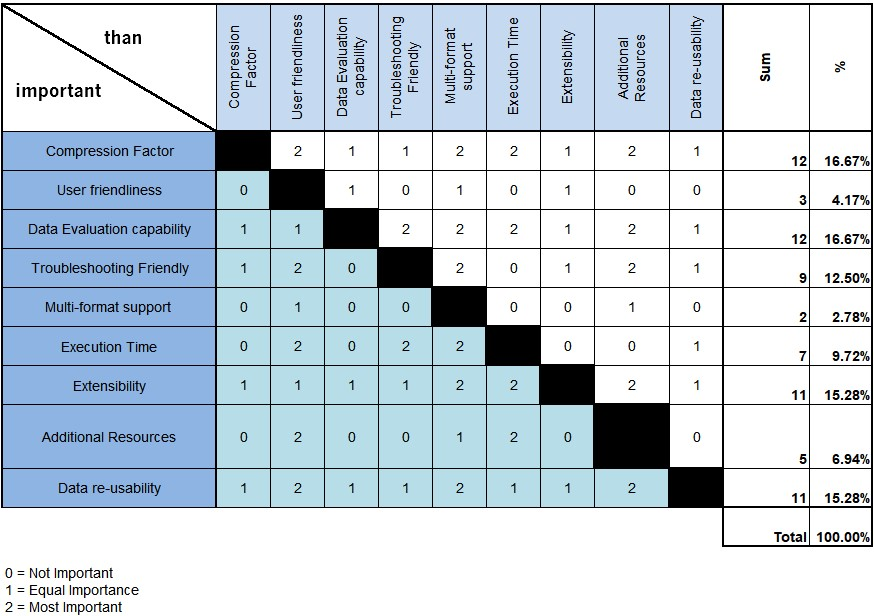
\includegraphics[width= 0.9\textwidth]{images/Paarweise.jpg}
    	\caption [Pairwise Comparison]{Pairwise Comparison}  
    	\label{fig:Pairwise Comparison}
\end{figure}

In the above figure, the pairwise comparison is conducted to determine the weightage of the requirements. This method enables the user to determine the priority of requirements for product development. As shown in the figure, the requirements are compared with each other and a 3 step priority marker is used to aid this comparison. 0 ,1 and 2 are the three indicators of priority with increasing priority compared with each other. Consider, the row Compression Factor where it is compared with 8 other requirements to determine it's weightage. Compression Factor is determined to be more important than the following factors : 1) User Friendliness 2) Multi-Format Support 3) Execution Time 4) Additional Resources. Whereas compared to the following requirements : 1) Data Evaluation Capability 2) Troubleshooting Friendly 3) Extensibility 4) Data Re-usability , the requirement Compression Factor is given equal importance. This is very intuitive and easy to understand in the sense that the key feature of a Data compression algorithm which is Compression Factor is given more importance over factors like User Friendliness, Multi file support, Execution Time and Additional Resources.

Any of the above four requirements can be compromised or rather given a lower priority of execution in order to achieve better compression rate. For e.g the outcome of the pairwise comparison will help determine an algorithm for data compression of .asc files. It might not be feasible to develop an algorithm that could achieve best compression for both .blf and .asc file types. Since, it is already determined that .blf files have very limited flexibility in terms of application of a data compression algorithm on it, priority could be given to the compression factor as a requirement and an algorithm could be selected which provides the highest compression for .asc files. Thus a higher importance is given to Compression Factor than to Multi format support. Similar parallels could be drawn to Compression Factor vs Execution time , Compression Factor vs Additional resources etc.

At the end of pairwise comparison compression factor and data evaluation capability achieve highest priority amongst all requirements, which is validated by the goal of this thesis. Extensibility or expand-ability of the algorithm and Data re-usability ,i.e ability to make use of values post compression, come close second. The percentage column is of great significance here. Until now, the pairwise comparison was used to determine which requirements should be assigned higher priority in product development cycle. Once the priorities of each requirements are determined, the next step is determine which algorithm is valid and imbibes the result of the pairwise comparison in itself. Weighted Analysis of algorithms helps in achieving this goal. The percentage column derived from pairwise comparison is also a metric which can be used in the weighted analysis. At the end of weighted analysis comparison, one out of five algorithms would be selected which is the closest to fulfilling all the requirements set in this thesis. 

\begin{figure}[!h]
    	\centering
    	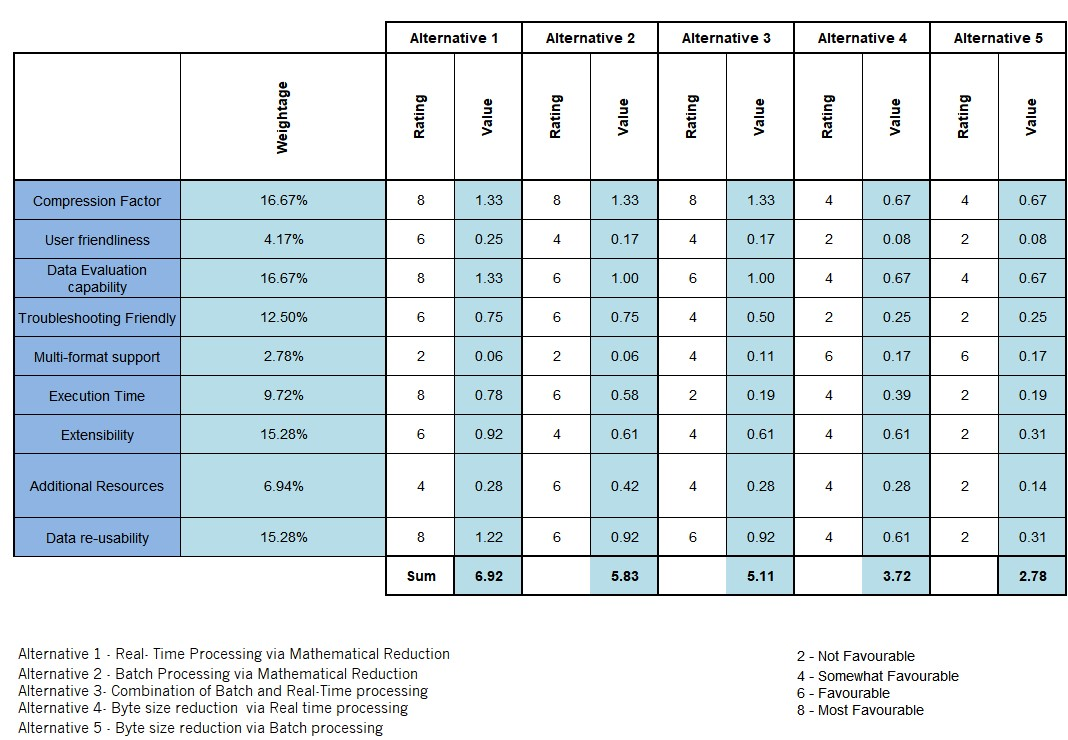
\includegraphics[width= 1\textwidth]{images/Weighted Analysis.jpg}
    	\caption [Weighted Analysis]{Weighted analysis}  
    	\label{fig:Weighted Analysis}
\end{figure}

The above diagram indicates the weighted analysis of all the 5 possible algorithms to achieve data compression on .asc files. The 5 algorithms are described as 5 alternatives in the above diagram. Compared to pairwise comparison, the rating, here, is not done on basis of priority instead the rating is symbolic of the property of the algorithm. There are 4 levels of Rating selected for each algorithms: from 2 all the way to 8. 2 is the least favourable rating which indicates that a particular requirement is not fulfilled by the algorithm. Whereas 8 indicates most favourable rating which indicates that for a particular requirement, the algorithm is the best fit. The following formula is used to calculate the weighted value assigned to each requirement fulfilling capability of the algorithm :
\begin{equation}
 Value (V)  = Weightage * Rating
\end{equation}
The Sum is the summation of all the weighted values : $\Sigma(Vn)$ . 

Each algorithm has it's own unique characteristics and the weighted analysis is a great method to showcase it's uniqueness. For example, alternative 1, 2 \& 3 all use the same mathematical model of arithmetic mean combined with filtering to achieve compression hence they have similar ratings for compression factor. However, there is a stark contrast in the three alternative when looking at a feature like execution time. Alternative 1 involves real time processing, hence the total execution time, calculated from test start to generation of reduced log file, is the lowest. Alternative 2 needs log files to be generated in order to perform compression in post processing approach, hence the execution time is increased in comparison to alternative 1. Alternative 3 uses a combination of both the alternative 1 \& 2, hence the total execution is greater than alternative 1 and 2. Thus, alternative 3 is the least suitable from the perspective of execution time as a key feature of the algorithm. 

At the end of weighted analysis, the algorithm with highest valuation wins. This means that the algorithm with the highest valuation is the most appropriate suit for all the defined requirements. As per \ref{fig:Weighted Analysis}, the alternative 1 has the highest valuation followed by alternative 2. The alternatives 4 and 5 have received the least valuations owing to various unsuitable factors such as :

\begin{itemize}
    \item Low compression factor : compared to mathematical model byte size reduction method is not very robust as it is heavily dependent on repetition of values
    \item User friendliness : complexity of the algorithm design and execution makes it unfavourable for the end user to use it intuitively
    \item Data evaluation capability : Due to encoding method used to implement these algorithms, it is possible data re-usability is drastically reduced which would in turn make data evaluation difficult
\end{itemize}

The sole feature where alternative 4 \& 5 outshine the other three alternatives are it's support for multi format file support. It is, theoretically, possible to implement these algorithms on both .asc and .blf files. However, the complexity that accompanies with practically implementing these methods outweighs the benefits they provide by offering multi file support. 


Hence, at the end of this study, it can be concluded that a mathematical reduction method accompanied with filtering or clipping is the most suitable approach for reducing the data-sets concerned with this thesis. The approach of real-time processing along-with mathematical reduction provides the best possible compression algorithm. Every scientific approach requires alternatives in case the most suitable approach hits a bottleneck due to unforeseen scenarios. In such scenarios, batch processing along-with mathematical reduction is a relevant alternative coming close second in the weighted analysis study of all the algorithms. 		% 4. ...
\newpage

\thispagestyle{myPageStyle}
% Kapitel 9 - Fazit
\section{Implementation}
In chapter \ref{sec:Algorithm definition}, a comprehensive and exhaustive study of different approaches to compression algorithm was conducted. The conclusion drawn was that an approach with mathematical reduction with a combination of data filtering was the most suitable for the type of data-sets being dealt with in this thesis, i.e .asc files. In this chapter, the implementation of the conclusion from previous chapter would be discussed.

\subsection{Algorithm Selection}
As per figure \ref{fig:Weighted Analysis}, real time processing via mathematical reduction is the most suitable method to achieve optimal fulfillment of the requirements. The implementation of this method requires to easy access to :

\begin{itemize}
    \item Test systems with CANoe pre-installed
    \item CAPL coding environment
    \item Data files for testing and validation
\end{itemize}

CANoe is a licensed tool provided by Vector Informatik GmbH. It is a complex and large tool to use with numerous features suitable for different types of uses in diversified environments in the domain of verification \& validation. The licenses are extremely expensive and hence the easy access to such tools is also restricted. Usually such licenses are purchased in limited quantities and shared in team pools for various projects and hence the access is always determined by priority of implementation basis. 

Vector provides three types of licensing for CANoe tool, each of which have their own utilities and limitations. The three types of licenses are :

\begin{itemize}
    \item CANoe pro
    \item CANoe run
    \item CANoe pex
\end{itemize}

The pro version is the highest tier license version of CANoe. As the name suggests, the license gives access to all features of CANoe tool which also includes CAPL coding environment. The run license provides limited access to CANoe environment where it is possible to run and analyse all the pre-existing test setups and programs. The user is restricted from changing any configurations in the setups using run license. The pex license is the basic license required to view CANoe tool. It is useful for viewing the tool and it's setup and configurations, however, creating, running or changing configurations and setups are prohibited. Here, \ref{fig:CANoe Licenses}, one can see the features included with pro license.

\begin{figure}[h]
    	\centering
    	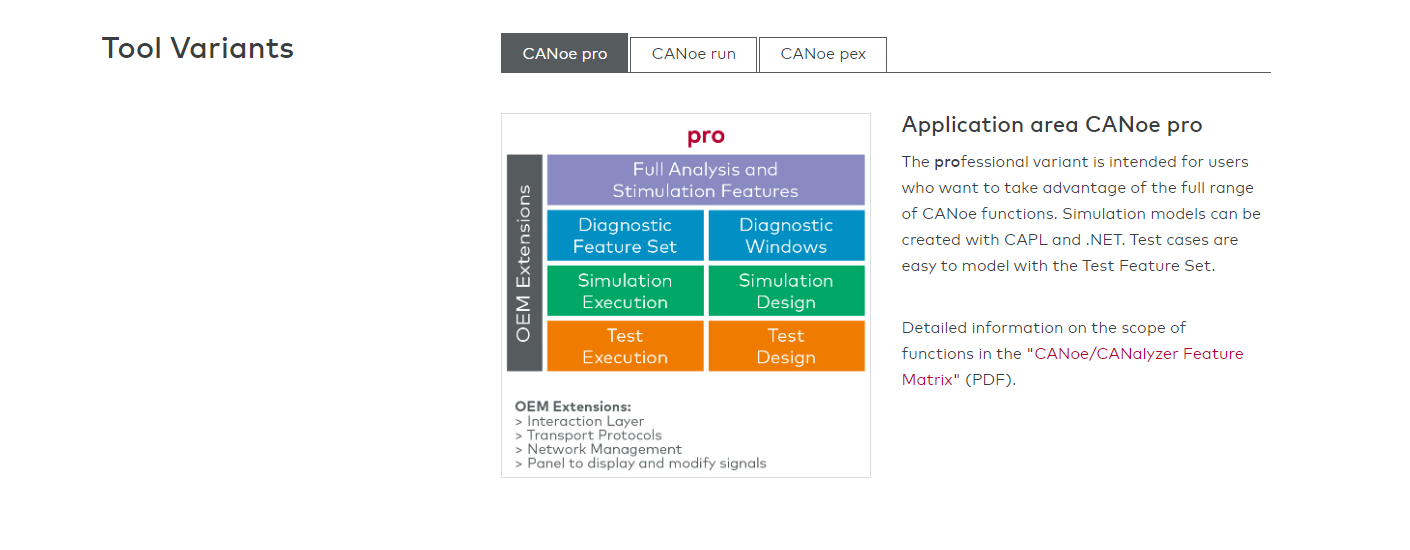
\includegraphics[width= 1\textwidth]{images/CANoe license type.png}
    	\caption [Licenses]{CANoe licenses}  
    	\label{fig:CANoe Licenses}
\end{figure}

\begin{figure}[h]
    	\centering
    	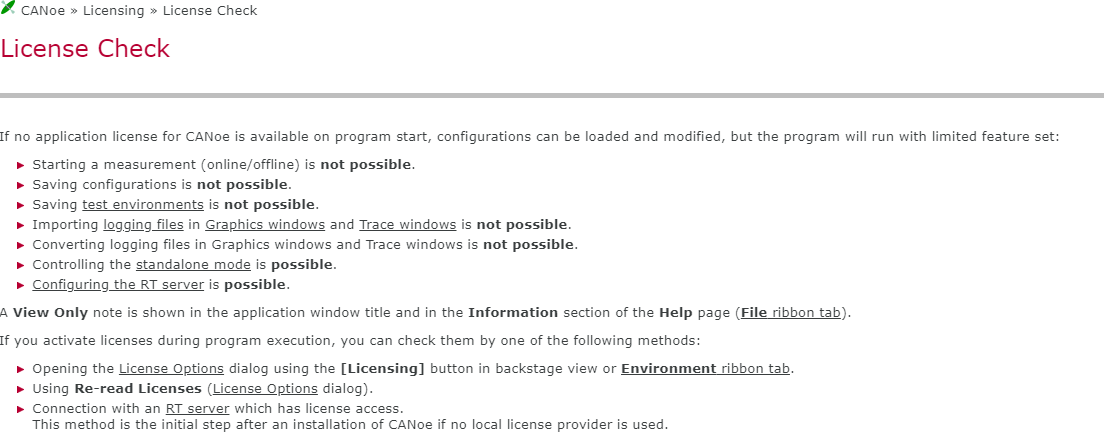
\includegraphics[width= 1\textwidth]{images/CANoe license restrictions.png}
    	\caption [Restrictions]{CANoe restrictions}  
    	\label{fig:CANoe Restrictions}
\end{figure}


\clearpage

Figure \ref{fig:CANoe Restrictions} shows the restrictions involved with limited access licenses. Hence, it is of utmost importance to have access to the pro version of licenses. At CES, CANoe pro licenses are available to use for test systems. However, it is subjected to availability of the test systems. Since, multiple projects require the availability of test systems, getting a free-to-use access to test systems is difficult. Since, implementing the algorithm requires constant access to development environment for development, testing and validation an alternative was required to overcome the limited access to the test systems. 

As discussed in the conclusion of \ref{sec:Algorithm definition}, the weighted analysis revealed two possible alternatives for implementation of mathematical reduction based compression algorithm : \\
1) Real Time Processing    2) Batch Processing or Post-Processing 

Since, the approach for compressing data and reducing data size in both processes is identical, the use of an alternative to the real time processing approach can be considered and tested to verify if the desired compression is achieved or not. Once, the data compression is verified and validated, the algorithm can be transferred from post-processing to real-time processing with necessary changes. This will be discussed as part of scope of development for future.

To conclude, the compression algorithm with post processing will be used as the base for implementation study and the development platform to be used for this purpose will be python.

But before moving to development phase, it is necessary to define the structure of the program. Without a proper structure, it is easy to lose the sight of goal or worse get entangled in unproductive development hassles irrelevant to the goals. Designing the structure of a program before starting to code is an important step in the software development process. It can help ensure that the code is well-organized, maintainable, and easy to understand. Here are some common ways to design the structure of a program: 

\begin{itemize}
    \item Pseudocode: Pseudocode is a high-level, human-readable description of the steps a program should take to solve a problem. It is written in a syntax that resembles a programming language but is not meant to be executed. Pseudocode can be a useful tool for designing the structure of a program, as it allows you to think through the problem and get a rough idea of the steps your code will need to take before writing any actual code.
    \item Flowcharts: Flowcharts are diagrams that show the flow of control through a program. They can be used to represent the structure of a program, making it easy to see the different parts of the program and how they relate to each other. Flowcharts can be a helpful tool for designing complex programs, as they make it easy to see the logic of the program at a high level.
    \item Mind maps: Mind maps are diagrams that show the relationships between different ideas or concepts. They can be used to design the structure of a program by breaking the problem down into smaller parts and showing how they fit together. Mind maps can be a good way to get a bird's eye view of the program and see how all of the pieces fit together.
    \item Diagrams and schematics: You can also use other types of diagrams and schematics to design the structure of a program. For example, you might use a block diagram to show the relationships between different parts of the program, or a state diagram to show the different states that a program can be in and the transitions between those states.
    \item Code sketching: Finally, you can also start designing the structure of a program by sketching out some of the code on paper. This can be a good way to experiment with different approaches and see what code structures make the most sense for the problem you are trying to solve.
\end{itemize}

\newpage
\subsection{Initial Setup}

Python is a high-level, interpreted, general-purpose programming language. It was first released in 1991 by Guido van Rossum and has since become one of the most widely used programming languages in the world.

Python is popular for its simple, easy-to-read syntax which allows developers to express concepts in fewer lines of code compared to other programming languages. It is also highly versatile and can be used for a variety of applications, including web development, scientific computing, data analysis, artificial intelligence, and more. One of the main benefits of using Python is its extensive library of modules and packages, which makes it easy to perform common programming tasks without having to write extensive amounts of code. This has led to a large and active community of developers who continuously contribute to the development and improvement of the language.

There are currently two stable versions of Python in widespread use: Python 2 and Python 3. Python 2 was first released in 2000, and although it is still in use, its development has been largely discontinued in favor of Python 3. Python 3 was first released in 2008 and has since become the standard version of Python, with many improvements over Python 2. The compression algorithm discussed in this thesis has thus been designed exclusively using Python 3. 

Python programs can be written and executed by means of a terminal or IDE also known as Integrated development environment. The scripts, or codes, are written and saved with a ".py" extension. An IDE was selected and utilized for the purpose of development of compression algorithm in this thesis. An integrated development environment (IDE) is a software application that provides comprehensive facilities to computer programmers for software development. An IDE normally consists of at least a source code editor, build automation tools and a debugger \cite{PyWiki}. IDEs maximize user productivity by providing easy access to multiple components of the coding environment such as code alignment, errors \& warnings indicators, easy install of packages library etc.   

One aim of the IDE is to reduce the configuration necessary to piece together multiple development utilities. Instead, it provides the same set of capabilities as one cohesive unit. Reducing setup time can increase developer productivity, especially in cases where learning to use the IDE is faster than manually integrating and learning all of the individual tools. Tighter integration of all development tasks has the potential to improve overall productivity beyond just helping with setup tasks. For example, code can be continuously parsed while it is being edited, providing instant feedback when syntax errors are introduced, thus allowing developers to debug code much faster and more easily with an IDE.

Some IDEs are dedicated to a specific programming language, allowing a feature set that most closely matches the programming paradigms of the language.\cite{PyWiki} PyCharm is one such IDE dedicated for the development of python based programs. It provides code analysis, a graphical debugger, an integrated unit tester, integration with version control systems, and supports web development with Django. It is cross-platform, working on Microsoft Windows, macOS and Linux. PyCharm has two editions : Professional and Community. PyCharm Community Edition is less extensive than the Professional Edition. While PyCharm professional is suited for both scientific and web python development with HTML, JS and SQL support at a subscription price, PyCharm Community edition is a free version for pure python development aimed at hobbyist or beginners who want to develop programs without integration to web. For the purpose of this thesis, the PyCharm Community Edition is used since web based development is not involved here. Below is a representation of the PyCharm IDE interface:

\begin{figure}[h]
    	\centering
    	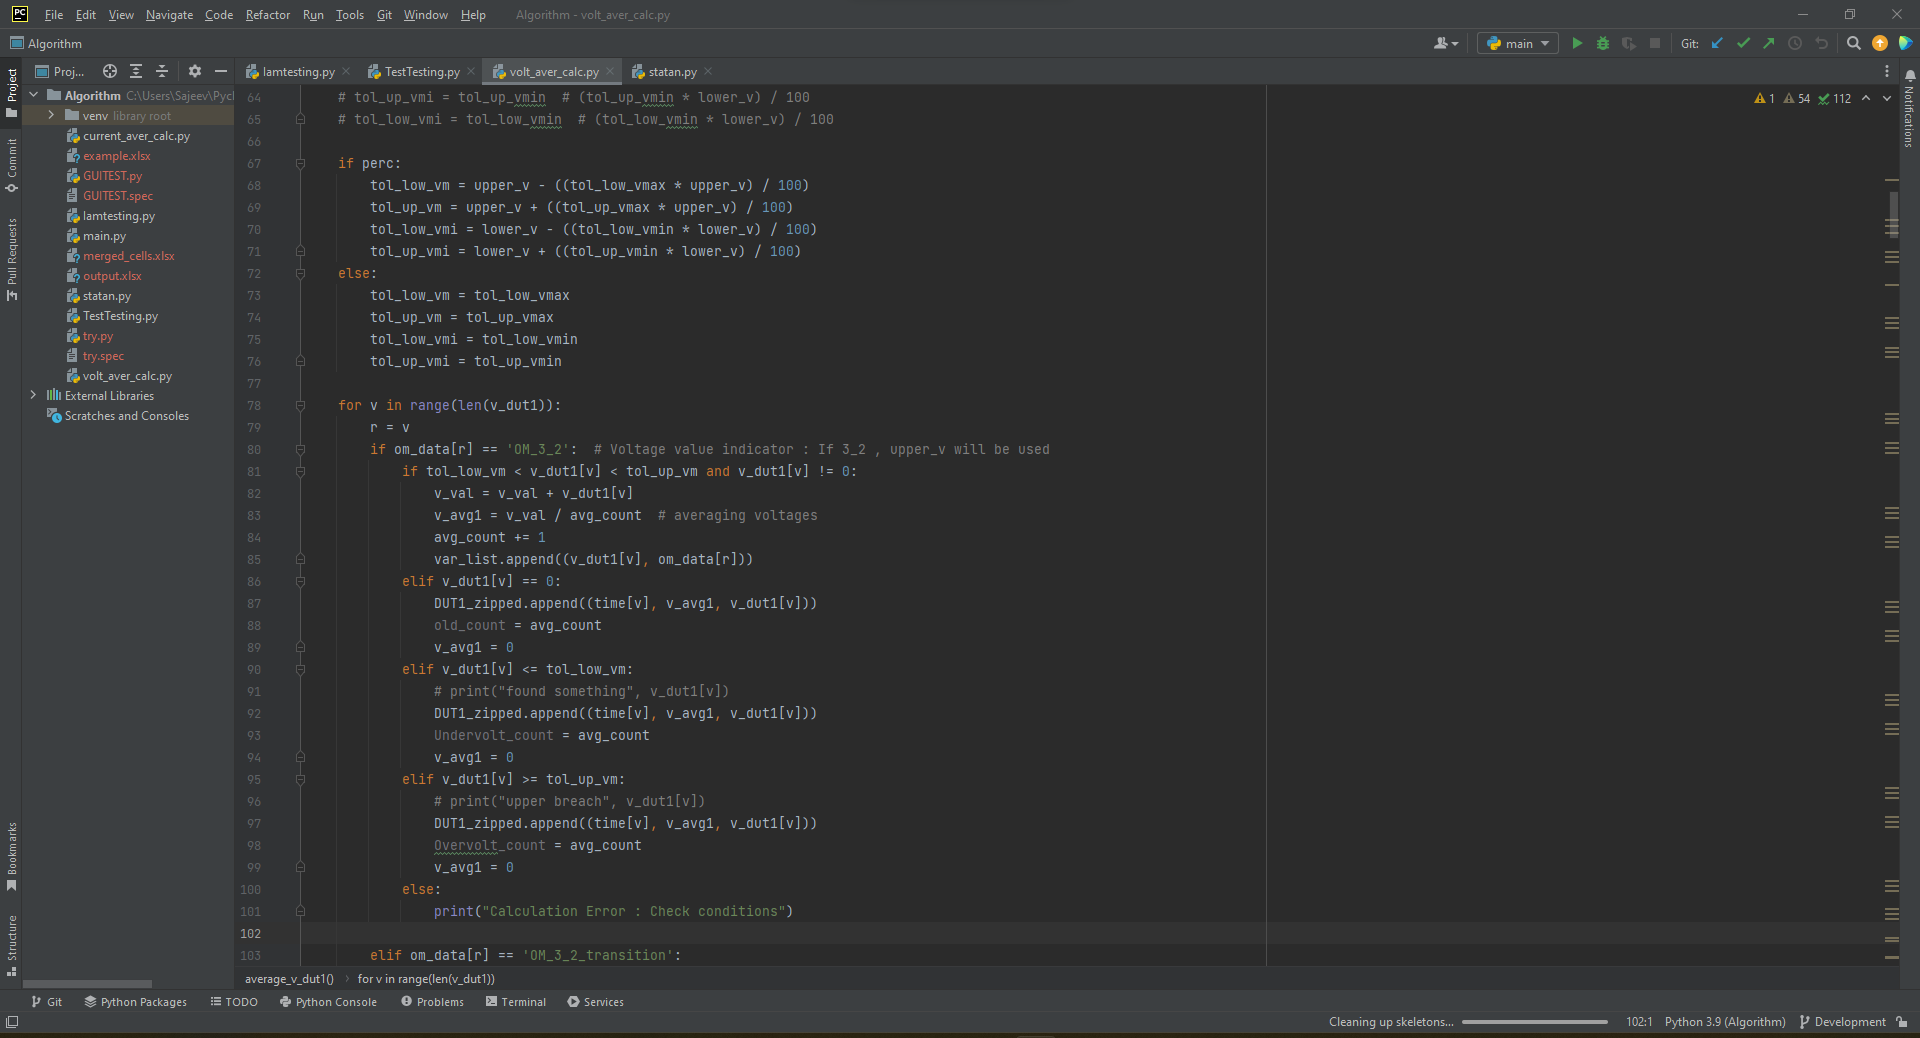
\includegraphics[width= 1\textwidth]{images/pycharm.png}
    	\caption [PyCharm]{PyCharm Interface}  
    	\label{fig:Pycharm interface}
\end{figure}



\newpage
    
\subsection{Einschränkungen}


\paragraph{Evaluation} 
Bla bla.

\paragraph{Konzept}


%\input{chap9x} %chap9_futurework_limitations}			% 5. ...
\newpage

\thispagestyle{myPageStyle}
\section{Concluding Discussions} 

\subsection{Conclusive Summarization} 
This thesis started with discussions about automotive systems and the testing of automotive components followed by a discussion about the importance of testing. This discussion shed a light on the outcome of testing and the data-files or logs associated with it. The storage and size of data-files were determined as a deterrent or Achilles heel for efficient handling, evaluation and preservation of test datas. 

It was thus necessary to conduct a study about what these data-logs exactly are and what are the problems and necessary solutions associated with storing them. Thus, came data compression into picture. Further on, focus was placed on studying different data compression methods and determining which type of method suited best for the data-logs studied in the context of this thesis. After a comprehensive study, it was determined that from the two types of data-logs studied in this thesis, one of the data-logs using ".blf" could be compressed only by method of zipping. The maximum compression ratio achievable by this method depends on the zipping software or algorithm used. Studies on this topic, thus, didn't result in very promising results.

However, the data-logs also consist of ".asc" files and the studies in direction of compression/reduction of file size of this datatype were relatively more successful. 5 different compression techniques could be derived for these file types. A QFD based study and weighted analysis helped in selecting the best possible theoretical solution for compressing data-files of ".asc" type. In practical implementation, a slight deviation from the theoretical solution was observed due to time and resource constraints. Although it was a deviation, the principle implementation was exactly the same and the logic behind it too with only the platform of implementation changing from proprietary tool to a more conventional tool called Python. Once the implementation started multiple trial and error rounds were conducted before finalising the desired algorithm implementation on these data-files.

The algorithm was able to keep up with the requirements set at the beginning of this thesis. There were significant improvements in compressing the file sizes of the logs. At times, in ideal test run scenarios a compression of up-to 97\% could also be observed. The algorithm also achieved data evaluation goals set in the beginning. Thus, to conclude it can be stated that a successful study of problems, possible solutions and ultimately testing out the optimal solution for the target subject was conducted by means of this thesis.


\newpage

\subsection{Scope for future improvisations}

There is never a dearth for improvements when it comes to innovation and technology. It's only with improvisations, the best out of a concept can be extracted and delivered to make the best possible product ever.  Thus, it is only appropriate to also discuss the same in context with this thesis. 

\begin{itemize}
    \item Parallel Processing :- The algorithm must be implemented with the same program design on to the test system based proprietary tool CANoe to achieve more functionality as parallel processing would provide the program easy access to various system variables and that greatly increases the degree of freedom while designing the algorithm.

    \item Improved Data Evaluation :- A different approach to drift analysis could be implemented, possibly over the whole duration of the test run. This would give more idea of all the drifts involved in the DUTs. 

    \item Advanced algorithm  :- The algorithm could be enhanced or altered to involve compression of ".blf" files as well. Studying the contents of ".blf" files individually and then integrating a compression algorithm for those could be a work in the right direction. Also, it is worth considering if the system explicitly ".blf" files and then a compression algorithm is run on to it and then ".asc" file is generated from this compressed ".blf" file in order to achieve overall compression.

    \item Less customised approach :- A more generalised approach in terms of user inputs, test definitions and monitoring conditions could be tried and tested so that in future regardless of the test-system or test-design, the algorithm could be universally implemented, at-least with respect to test systems at CES. 
    
\end{itemize}			% 6. Study design and execution
\newpage

\thispagestyle{myPageStyle}
\input{Chapter7/chap7}			% 7. Evaluation and Results
\newpage
\fi

\thispagestyle{myPageStyle}
% Kapitel 8 - Diskussion
\section{Diskussion}
Diskussion der Resultate im Vergleich zu Ergebnissen der Related work-Analyse und Reflektion auf die Forschungsfragen/Hypothesen.

Hypothese \textbf{H1} kann angenommen werden. Bla bla Begründung/Argumentation.

Andererseits zeigen die Ergebnisse der Evaluation aber keinen signifikanten Unterschied (siehe \cite{field}) zwischen X und Y - somit kann auch \textbf{H2} angenommen werden. Da hier bla bla Argumentation.

Durch die Ergebnisse des Fragebogens wird Hypothese \textbf{H3} nicht bestätigt. Es sind keine signifikanten Unterschiede über die ... 


			% 8. Discussion, Deriving concrete action recommendations
\newpage

\thispagestyle{myPageStyle}	% 9. Conclusion, Future work, Limitations
% Kapitel 9 - Fazit
\section{Fazit}
Diese Arbeit befasste sich grundsätzlich mit der Frage, welche Anforderungen an ... gestellt werden.
Der Lösungsvorschlag war...
Benutzerstudien haben gezeigt, dass es einen signifikanten Unterschied... gibt. Diese Ergebnisse motivieren, um ...

\subsection{Ausblick} 
In dieser Arbeit haben wir uns mit ... beschäftigt. Durch zwei Benutzerstudien wurde festgestellt, dass sich die Aufteilung und Positionierung der Informationen innerhalb der Anzeige der beiden Gruppen aufgrund bla bla ändert. Das entwickelte Konzept ist zwar bla bla, müsste aber für eine Wiederholung der Studien bla bla zur Erhebung quantitativer Daten wie folgt angepasst werden:

\begin{itemize}
\item xxx
\item yyy
\item xzz
\end{itemize}

Des Weiteren wurde festgestellt, dass bla bla. Auch das müssten zukünftige Varianten besser berücksichtigen, z.\,B., indem sie bla bla. Für Studien sollte zudem eine neutrale(re) Umgebung gewählt werden. Somit sollte sichergestellt werden können, dass beispielsweise ein möglicher Bias der Marke des Fahrzeugs sich nicht auf das HMI-Konzept auswirkt...

\subsection{Einschränkungen}
Hinsichtlich Einschränkungen, die eine breite Anwendung der Ergebnisse verhindern, sind zwei getrennte Bereiche zu betrachten. Zum einen die Evaluation, welche sich nur auf den ersten Teil der Arbeit bezieht, zum anderen das ausgearbeitete Konzept für die Anzeige, das auf dem ersten Teil der Arbeit aufbaut. \\ [-2.5em]

\paragraph{Evaluation} 
Bla bla.

\paragraph{Konzept}
Bla bla. Das wurde etwa in beschrieben...

%\input{chap9x} %chap9_futurework_limitations}
\newpage	

	%\shorthandon{"}
	
%--------------------------------------------------------------------------------
%-----Anhang---------------------------------------------------------------------
%--------------------------------------------------------------------------------
	
	\pagenumbering{Roman} 					% Römische Nummerierung der Kapitel/Roman page numbering
	\setcounter{page}{6} 						% Beginn bei Seitenzahl X (hier: 6) um bei oberer Nummerierung aufzuschließen/Adapt page numbering
	
	%Glossar/Glossary
	\thispagestyle{myPageStyle}
	\glssetwidest{A D A S} 						% gleicher Abstand zur 2. Spalte (längstes Wort)					
	\setglossarystyle{alttree}																	
	%\printglossary[title=Abkürzungsverzeichnis,toctitle=Abkürzungsverzeichnis] 	% Rename for German thesis
	\cleardoublepage
		
	
	%Literaturliste/Literature references
	\thispagestyle{myPageStyle}
	\bibliographystyle{plainnat}
	%\bibliographystyle{abbrv}% changed abbrvdin to abbrv % DIN-Norm für Literaturdarstellung  plaindin 
	%\bibliographystyle{abbrvnat}
	\setcitestyle{authoryear, open={(}, close={)}}
	
	\renewcommand{\refname}{Literature references} % Remove for German thesis
	\bibliography{literature}					% Pfad und Datei der Literaturdatenbank/Path and file name of literature references
	\cleardoublepage	
	
	%Anhänge/Appendices
	%\thispagestyle{myPageStyle} 
	%%----------Anhang/Appendices--------------------------------------------------------------

\appendix
\section{Anhang}

\subsection[]{Onlinefragebogen} \label{sec:a1} 
%\vspace{2em}
%\includepdf[pages={2-3}]{images/fragebogen/questionnaire2}

\subsection[]{Rohdaten des Onlinefragebogens für die statistische Auswertung}

\subsection[]{Auswertung der Evaluation hinsichtlich...}

\subsection[]{Datenträger/Data carrier}
	%\cleardoublepage
	
%----------------------------------------------------------------------------------
%----------------DOKUMENTENENDE - END OF DOCUMENT----------------------------------
%----------------------------------------------------------------------------------
	
\end{document}